%
% This file is part of ICTP RegCM model.
% Copyright (C) 2011 ICTP Trieste
% See the file COPYING for copying conditions.
%
\documentclass[10pt,twoside,a4paper]{report}
\usepackage{natbib}
\usepackage{graphicx}
\usepackage{fancyvrb}
\usepackage{wrapfig}

\citestyle{apalike}

\begin{document}

\begin{titlepage}

\begin{wrapfigure}{l}{4cm}
\vspace{-35pt}
\begin{center}

\includegraphics{ICTP_logo}
\end{center}
\end{wrapfigure}

\noindent {\bf The Abdus Salam }\\
\noindent {\bf International Centre for Theoretical Physics} \\
\noindent {\bf Strada Costiera, 11 I - 34151 Trieste, Italy} \\
\noindent {\bf Earth System Physics Section - ESP}

\vspace{3cm}

\begin{center}
\noindent{{\Large
  {\bf Regional Climatic Model RegCM User's Guide} \\
  {\bf Version 4.1} \\
  {\bf Trieste, Italy - May 2011}
}}
\end{center}
\begin{center}
\noindent{\small{
\bf Filippo Giorgi, Nellie Elguindi, \\
    Stefano Cozzini and Graziano Giuliani
}} \\
\end{center}

\end{titlepage}

\cleardoublepage

\tableofcontents

\cleardoublepage

\chapter{Release Notes}
%%::::::::::::::::::::::::::::::::::::::::::::::::::::::::::::::::::::::::::::::
%%
%%    This file is part of ICTP RegCM.
%%    
%%    Use of this source code is governed by an MIT-style license that can
%%    be found in the LICENSE file or at
%%
%%         https://opensource.org/licenses/MIT.
%%
%%    ICTP RegCM is distributed in the hope that it will be useful,
%%    but WITHOUT ANY WARRANTY; without even the implied warranty of
%%    MERCHANTABILITY or FITNESS FOR A PARTICULAR PURPOSE.
%%
%%::::::::::::::::::::::::::::::::::::::::::::::::::::::::::::::::::::::::::::::

The Regional Climate Model developed at ICTP has now reached its 5.0 release.
The code base is actively developed by a community of developers internal and
external to ICTP, and this work is merged on the GitHub site.

The main new technical features of the release 5.0 are summarized in the
following points:

\begin{itemize}
  \item A new fast non-hydrostatical core derived from CNR MOLOCH has
      been added, and now RegCM has three different dynamical cores.
  \item The CMIP6 Input4MIPS dataset is now used by the RegCM in its
      original format, and climatological (MERRA2) and Simple Plume model
      data can be used as non interactive aerosol for the radiation code.
  \item The ERA5 and CMIP6 data from a number of different GCMs are now
      supported.
\end{itemize}
For the list of fixed bug, please refer to the git log.

The model code is in Fortran 2003 ANSI standard.
The development is done on Linux boxes and porting effort will be invested
toward porting the model on non Unix-like Operating Systems.
We will for this User Guide assume that the reference platform is a recent
Linux distributon with a \verb=bash= shell.
Typographical convention is the following:

\begin{table}[ht]
\caption{Conventions}
\vspace{0.05 in}
\centering
\begin{tabular}{l|l}
\hline
\verb=$> = & normal shell prompt \\
\verb=#> = & root shell prompt \\
\verb=$SHELL_VARIABLE = & a shell variable \\
\hline
\end{tabular}
\label{conventions}
\end{table}

Any shell variable is supposed to be set by the User with the following example
syntax:

\begin{Verbatim}
$> export REGCM_ROOT="/home/user/RegCM"
\end{Verbatim}

Hope you will find this document useful. Any error found belongs to the
RegCNET and can be reported to be corrected in future revisions. Enjoy.


\chapter{Obtain the model}
%
% This file is part of ICTP RegCM model.
% Copyright (C) 2011 ICTP Trieste
% See the file COPYING for copying conditions.
%

\section{Simple Model User}

A packed archive file with the model code can be downloaded from:

\begin{Verbatim}
http://gforge.ictp.it/gf/project/regcm/frs
\end{Verbatim}

and it can be later on decompressed and unpacked using:

\begin{Verbatim}
$> tar -zxvf RegCM-4.5.0.tar.gz
\end{Verbatim}

\section{Model Developer}

If you plan to become a model developer, source code can be obtained via svn.
The RegCM team strongly encourages the contributing developers to enroll on
the gforge site to always be up to date and to check on-line all the news of
the package.

\vspace{0.5cm}
\begin{tabular}{|c|}
\hline
{\bf https://gforge.ictp.it/gf/project/regcm} \\
\hline
\end{tabular}
\vspace{0.5cm}

The correct procedure is first to register on the G-forge site, then ask
the ICTP scientific team head Filippo Giorgi to be enrolled as a model
developer. After being officially granted the status, you will gain
access to the model subversion repository.

Check that {\bf Subversion} software is installed on your machine typing
the following command:

\begin{verbatim}
$> svn --version
\end{verbatim}

If your system answers \verb=command not found=, refer to your System
Administrator or software installation manual of your OS to install the
subversion software. As an example, on Scientific Linux the command
to install it as root is:

\begin{verbatim}
#> yum install subversion
\end{verbatim}

If Subversion is installed, after enrolled just type the following command:

\begin{verbatim}
$> svn checkout https://gforge.ictp.it/svn/regcm/branches/regcm-core
\end{verbatim}

To setup the model code from the SVN for your system, run the
\verb=bootstrap.sh= script:

\begin{verbatim}
$> ./bootstrap.sh
\end{verbatim}

The system must have installed the \verb=autoconf=, \verb=automake= and
\verb=libtool= programs.


\chapter{Installing procedure}
\label{install}
%
% This file is part of ICTP RegCM model.
% Copyright (C) 2011 ICTP Trieste
% See the file COPYING for copying conditions.
%

Whatever method is chosen to download the code, we assume that you have now
on your working directory a new directory, named \verb=RegCM-4.3=.
That directory will be for the rest of this guide referred as 
\verb=$REGCM_ROOT= .

All the operations to build the model binaries will be performed in this
directory.

\section{Software requirements}

In order to configure and install the RegCM code, the following software are
needed:

\begin{enumerate}
\item Python 2 language interpreter
\item GNU Make program
\item Fortran 2003 compiler
\item netCDF \cite{Rew_90} Format I/O library compiled with the above compiler.
   Source code can be found from \\
{\bf ftp://ftp.unidata.ucar.edu/pub/netcdf/netcdf.tar.gz} \\
Note that current netCDF version 4.2 is dependent on HDF5 1.8.8.
\end{enumerate}

Optional requirements strongly suggested are :

\begin{enumerate}
\item GNU \verb=patch= program if CLM option is activated.
\item MPI2 Message Passing Library compiled with the above fortran compiler
for parallel runs using multiple core single machines or cluster of machines.
Source code for the implementation code was tested with can be obtained at: \\
{\bf http://www.open-mpi.org/software/ompi/v1.4/downloads}
\item HDF5 Format I/O Library compiled with the above fortran compiler to
enable netCDF V4 features. Source code can be obtained at: \\
{\bf http://www.hdfgroup.org/ftp/HDF5/current/src}
\item NCO netCDF Operators for manging netCDF file. Most Linux distribution
have this already packed, and you should refer to your System Administrator or
OS Software Installation manual to obtain it. Source code is at: \\
{\bf http://nco.sourceforge.net/src}
\item CDO Climatic data Operators for managing netCDF file. Most Linux
distribution have this already packed, and you should refer to your System
Administrator or OS Software Installation manual to obtain it.
Source code is at: \\
{\bf https://code.zmaw.de/projects/cdo/files}
\item A Scientific Plotting and Data Analysis Software such as:
\begin{itemize}
\item IGES GrADS 2.0 Graphical Analysis and Display System. Convenient helpers
are packed in RegCM to use GrADS with RegCM netCDF output files.
Binaries and source code can be obtained from \\
{\bf http://www.iges.org/grads/downloads.html}
\item NCL, NCAR CISL Command Language. The NCL can read netCDF output files, and
sample scripts can be found in the {\em Tools/Scripts/NCL} directory.
Binaries and source code can be obtained from \\
{\bf http://www.ncl.ucar.edu}
\end{itemize}
\item A quick viewer for netCDF files like NcView: \\
{\bf http://meteora.ucsd.edu/~pierce/ncview\_home\_page.html}
\end{enumerate}

An example session of installation of basic software needed to compile the
RegCM model is detailed in chapter $\ref{Appendice}$.

\section{Configuring build}

The RegCM Version 4.3 is configured by a python2 script, which will select
and edit for you sample configuration files for the supported architectures.
These files are kept in the \verb=Arch= directory under \verb=$REGCM_ROOT=.

Currently tested and supported configurations (OS/Compiler) are:

\begin{enumerate}
\item Linux with GNU gfortran compiler version $\ge 4.6$
\item Linux with Intel\texttrademark ifort compiler version $\ge 11.0$
\item Linux with Portland\texttrademark pgf95 compiler version $\ge 11.0$
\item Mac OsX\texttrademark with g95 compiler
\item IBM AIX\texttrademark with xlf2003 compiler
\item Oracle Solaris\texttrademark with Oracle Solaris Studio\texttrademark
compiler $\ge 12.0$
\end{enumerate}

The 4.3 version of the RegCM model relies on the standard GNU autotools to
configure and build the model code.

The first step is to change working directory to \verb=$REGCM_ROOT= and run the
\verb=configure= script giving as arguments the chosen compilers:

\begin{Verbatim}
$> cd $REGCM_ROOT
$> ./configure CC=icc FC=ifort
\end{Verbatim}

To know the list of arguments that can be given to the configure script, the
script can be launched with the \verb=--help= command line argument.

\begin{Verbatim}
$> ./configure --help
\end{Verbatim}

The useful arguments to successfully build the model are:

\begin{Verbatim}
  --with-netcdf           Path to NetCDF installation (default: NETCDF
                          environment)
  --with-hdf5             Path to HDF5 installation (default: HDF5
                          environment)
  --with-szip             Path to SZIP installation (default: SZIP
                          environment)
  CC=         C compiler command
  CFLAGS=     C compiler flags
  LDFLAGS=    linker flags, e.g. -L<lib dir> if you have libraries in a
              nonstandard directory <lib dir>
  LIBS=       libraries to pass to the linker, e.g. -l<library>
  CPPFLAGS=   (Objective) C/C++ preprocessor flags, e.g. -I<include dir> if
              you have headers in a nonstandard directory <include dir>
  CPP=        C preprocessor
  FC=         Fortran compiler command
  FCFLAGS=    Fortran compiler flags
  MPIFC=      MPI Fortran compiler command
\end{Verbatim}

\subsection{Model configuration at build stage}
\label{modconf}

\begin{enumerate}
\item Enable debug
\begin{Verbatim}
  --enable-debug          Enable debugging flags and per processor log file
\end{Verbatim}
If enabled, the model will be compiled using debug flags for the compiler,
which will allow the use of a debugger such as gdb. More diagnostics will
also be generated during model run.
The default is to build production binaries with all optimization flags
turned on.

\item Serial code using stub MPI library
\begin{Verbatim}
  --enable-mpiserial      Use the included MPI replacement library for single
                          processor
\end{Verbatim}
The model is coded to use an MPI2 library to run in parallel mode using
multiple cores/processors or run on a cluster. To enable instead a serial
compilation option, a stub MPI library with empty callbacks needs to be
compiled and linked to the executable.
The RegCM team strongly suggest to build MPI enabled model also on standalone
systems, to take advantage of the multicore capabilities of any modern
processor.
\item CLM option
\begin{Verbatim}
  --enable-clm            Supply this option if you plan on using CLM option.
\end{Verbatim}
This option switches off the default Land model of RegCM (derived from BATS1e),
and enables the use of the Community Land Model V3.5 inside RegCM. The default
is to use the RegCM BATS Land Model.
\footnote{The CLM option needs the GNU patch program to be installed.}
For the scope of the tutorial test run in chapter \ref{tutorial}, use the
default option.
\end{enumerate}

\section{Build the model executables}

Now that everything is hopefully configured, you may use the \verb=make=
program to build executables.

\begin{Verbatim}
$> make
\end{Verbatim}

This target will builds all model parts. 
The compilation is started in the whole model tree (PreProc, Main and PostProc).
Lot of messages will appear on screen, abd at the end all executables are built
int the source directories.
To copy them to the \verb=Bin= directory, esplicitly issue the command:

\begin{Verbatim}
$> make install
\end{Verbatim}

Congratulations! You can now go to next step and run a test simulation.

\newpage

\chapter{Access global datasets}
\label{obdata}
%
% This file is part of ICTP RegCM model.
% Copyright (C) 2011 ICTP Trieste
% See the file COPYING for copying conditions.
%

The first step to run a test simulation is to obtain static data to localize
model DOMAIN and Atmosphere and Ocean global model dataset to build initial
and boundary conditions ICBC to run a local area simulation.

ICTP maintains a public accessible web repository of datasets on:

{\bf http://clima-dods.ictp.it/data/d8/cordex }

We will in the following substitute this URL with a shell variable:

\begin{Verbatim}
$> export ICTP_DATASITE=http://clima-dods.ictp.it/data/d8/cordex
\end{Verbatim}

As of now you are requested to download required global data on your local disk
storage before any run attempt. In the future, the ICTP ESP team has
planned to make available an OpenDAP THREDDS Server to give remote access
to global dataset for creating DOMAIN and ICBC without the need to
download the global dataset, but just the required subset in space and time,
using the ICTP web server capabilities to create that subset.

\section{Global dataset directory Layout}

You are suggested to establish a convenient location for global datasets
on your local storage. Keep in mind that required space for a year of global
data can be as large as 8 GBytes.

Having this in mind, we will now consider that you the user have identified
on your system or have network access to such a storage resource to store say
100 GB of data, and have it reachable on your system under the
\verb=$REGCM_GLOBEDAT= location.
On this directory, you are required to make the following directories:

\begin{Verbatim}
$> cd $REGCM_GLOBEDAT
$> mkdir SURFACE CLM CLM45 SST EIN15
\end{Verbatim}

This does not fill all possible global data sources paths, but will be enough
for the scope of running the model for testing its capabilities.

\section{Static Surface Dataset}

The model needs to be localized on a particular DOMAIN. The needed information
are topography, land type classification and optionally lake depth (to run the
Hostetler lake model) and soil texture classification (to run the chemistry option
with DUST enabled).

This means downloading four files, which are global archives at $30 second$
horizontal resolution on a global latitude-longitude grid of the above data.

\begin{Verbatim}
$> cd $REGCM_GLOBEDAT
$> cd SURFACE
$> curl -o GTOPO_DEM_30s.nc ${ICTP_DATASITE}/SURFACE/GTOPO_DEM_30s.nc
$> curl -o GLCC_BATS_30s.nc ${ICTP_DATASITE}/SURFACE/GLCC_BATS_30s.nc
\end{Verbatim}

Optional Lake and Texture datasets:

\begin{Verbatim}
$> cd $REGCM_GLOBEDAT
$> cd SURFACE
$> curl -o ETOPO_BTM_30s.nc ${ICTP_DATASITE}/SURFACE/ETOPO_BTM_30s.nc
$> curl -o GLZB_SOIL_30s.nc ${ICTP_DATASITE}/SURFACE/GLZB_SOIL_30s.nc
\end{Verbatim}

\section{CLM Dataset}
\label{clmdata}

If you are planning to enable the \verb=CLM= option in the model, you will need
a series of files with global land surface characteristics datasets.

\begin{Verbatim}
$> cd $REGCM_GLOBEDAT
$> cd CLM
$> curl -o mksrf_fmax.nc ${ICTP_DATASITE}/CLM/mksrf_fmax.nc
$> curl -o mksrf_glacier.nc ${ICTP_DATASITE}/CLM/mksrf_glacier.nc
$> curl -o mksrf_lai.nc ${ICTP_DATASITE}/CLM/mksrf_lai.nc
$> curl -o mksrf_lanwat.nc ${ICTP_DATASITE}/CLM/mksrf_lanwat.nc
$> curl -o mksrf_navyoro_20min.nc ${ICTP_DATASITE}/CLM/mksrf_navyoro_20min.nc
$> curl -o mksrf_pft.nc ${ICTP_DATASITE}/CLM/mksrf_pft.nc
$> curl -o mksrf_soicol_clm2.nc ${ICTP_DATASITE}/CLM/mksrf_soicol_clm2.nc
$> curl -o mksrf_soitex.10level.nc ${ICTP_DATASITE}/CLM/mksrf_soitex.10level.nc
$> curl -o mksrf_urban.nc ${ICTP_DATASITE}/CLM/mksrf_urban.nc
$> curl -o pft-physiology.c070207 ${ICTP_DATASITE}/CLM/pft-physiology.c070207
$> curl -o pft-physiology.c070207.readme \
> ${ICTP_DATASITE}/CLM/pft-physiology.c070207.readme
$> curl -o rdirc.05.061026 ${ICTP_DATASITE}/CLM/rdirc.05.061026
\end{Verbatim}

This is the input file for the \verb=clm2rcm= program (see at \ref{clm}).

\section{CLM 4.5 Dataset}
\label{clm45data}

If you are planning to enable the \verb=CLM 4.5= option in the model, you will
need a series of files with global land surface characteristics datasets.

\begin{Verbatim}
$> cd $REGCM_GLOBEDAT
$> cd CLM45
$> mkdir megan pftdata snicardata surface
$> for dir in megan pftdata snicardata surface; do cd $dir; \
    wget ${ICTP_DATASITE}/CLM45/$dir/ -O - | \
    wget -A ".nc" -l1 --no-parent --base=${ICTP_DATASITE}/CLM45/$dir/ \
      -nd -Fri -; done
\end{Verbatim}

This is the input file for the \verb=mksurfdata= program (see at \ref{clm45}).

\section{Sea Surface Temperature}

The model needs a global SST dataset to feed the model with ocean temperature.
You have multiple choices for SST data, but we will for now for our test run
download just CAC OISST weekly for the period 1981 - present.

\begin{Verbatim}
$> cd $REGCM_GLOBEDAT
$> cd SST
$> CDCSITE="ftp.cdc.noaa.gov/pub/Datasets/noaa.oisst.v2"
$> curl -o sst.wkmean.1981-1989.nc \
> ftp://$CDCSITE/sst.wkmean.1981-1989.nc
$> curl -o sst.wkmean.1990-present.nc \
> ftp://$CDCSITE/sst.wkmean.1990-present.nc
\end{Verbatim}

\section{Atmosphere and Land temperature Global Dataset}

The model needs to build initial and boundary conditions for the regional scale,
interpolating on the RegCM grid the data from a Global Climatic Model output.
The GCM dataset can come from any of the supported models, but we will for now
for our test run download just the EIN15 dataset for the year 1990
(Jan 01 00:00:00 UTC to Dec 31 18:00:00 UTC)

\begin{Verbatim}
$> cd $REGCM_GLOBEDAT
$> cd EIN15
$> mkdir 1990
$> cd 1990
$> for type in "air hgt rhum uwnd vwnd"
>  do
>    for hh in "00 06 12 18"
>    do
>      curl -o ${type}.1990.${hh}.nc \
>         ${ICTP_DATASITE}/EIN15/1990/${type}.1990.${hh}.nc
>    done
>  done
\end{Verbatim}

With this datasets we are now ready to go through the RegCM Little Tutorial
in the next chapter of this User Guide.

\newpage

\chapter{Run a test simulation using the model}
\label{tutorial}
%
% This file is part of ICTP RegCM model.
% Copyright (C) 2011 ICTP Trieste
% See the file COPYING for copying conditions.
%

We will in this chapter go through a sample session in using the model with
a sample configuration file prepared for this task.

\section{Setting up the run environment}

The model executables prepared in chapter \ref{install} are waiting for us to
use them. So let's give them a chance.

The model test run proposed here requires around 100Mb of disk space to store
the DOMAIN and ICBC in input and the output files. We will assume here that you,
the user, have already established a convenient directory on a disk partition
with enough space identified in the following discussion with \verb=$REGCM_RUN=

We will setup in this directory a standard environment where the model can be
executed for the purpose of learning how to use it.

\begin{Verbatim}
$> cd $REGCM_RUN
$> mkdir input output
$> ln -sf $REGCM_ROOT/Bin .
$> cp $REGCM_ROOT/Testing/test_001.in .
$> cd $REGCM_RUN
\end{Verbatim}

Now we are ready to modify the input namelist file to reflect this directory
layout. A namelist file in Fortran90 is a convenient way to give input to a
program in a formatted file, read at runtime by the program to setup its
execution behaviour. So next step is somewhat tricky, as you need to edit
the namelist file respecting its well defined syntax. Open your preferred text
file editor and load the \verb=test_001.in= file. You will need to modify for
the scope of the present tutorial the following lines:

\begin{Verbatim}
FROM:
 dirter = '/set/this/to/where/your/domain/file/is',
TO:
 dirter = 'input/',
\end{Verbatim}

\begin{Verbatim}
FROM:
 inpter = '/set/this/to/where/your/surface/dataset/is',
TO:
 inpter = '$REGCM_GLOBEDAT',
\end{Verbatim}

where \verb=$REGCM_GLOBEDAT= is the directory where input data have been
downloaded in chapter \ref{obdata}.

\begin{Verbatim}
FROM:
 dirglob = '/set/this/to/where/your/icbc/for/model/is',
TO:
 dirglog = 'input/',
\end{Verbatim}

\begin{Verbatim}
FROM:
 inpglob = '/set/this/to/where/your/input/global/data/is',
TO:
 inpglob = '$REGCM_GLOBEDAT',
\end{Verbatim}

and last bits:

\begin{Verbatim}
FROM:
 dirout='/set/this/to/where/your/output/files/will/be/written'
TO:
 dirout='output/'
\end{Verbatim}

This modifications just reflect the above directory layout proposed for this
tutorial, and any of this paths can point anywhere on your system disks. Path
is limited to $256$ characters.
We are now ready to execute the first program of the RegCM model.

\section{Create the DOMAIN file using terrain}

First step is to create the DOMAIN file to localize the model on a world region.
The program which does this for you reading the global databases is
\verb=terrain= .

To launch the terrain program, enter the following commands:

\begin{Verbatim}
$> cd $REGCM_RUN
$> ./Bin/terrain test_001.in
\end{Verbatim}

If everything is correctly configured up to this point, the model should print
something on stdout, and the last lines will be:

\begin{Verbatim}
 Grid data written to output file                                               
 Successfully completed terrain fields generation
\end{Verbatim}

In the input directory the program will write the following two files:

\begin{Verbatim}
$> ls input
test_001_DOMAIN000.nc test_001_LANDUSE
\end{Verbatim}

The DOMAIN file contains the localized topography and landuse databases, as
well as projection informations and land sea mask. The second file is an ASCII
encoded version of the landuse, used for modifying it on request. We will cover
it's usage later on.  To have a quick look at DOMAIN file content, you may want
to use the GrADSNcPlot program:

\begin{Verbatim}
$> ./Bin/GrADSNcPlot input/test_001_DOMAIN000.nc
\end{Verbatim}

If not familiar with GrADS program, enter in sequence the following commands at
the \verb=ga->= prompt:

\begin{Verbatim}
ga-> q file
ga-> set gxout shaded
ga-> set mpdset hires
ga-> set cint 50
ga-> d topo
ga-> c
ga-> set cint 1
ga-> d landuse
ga-> quit
\end{Verbatim}

this will plot the topography and the landuse on the X11 window.

\section{Create the SST using the sst program}

We are now ready to create the Sea Surface Temperature for the model, reading a
global dataset.
The program which does this for you is the \verb=sst= program, which is executed
with the following commands:

\begin{Verbatim}
$> cd $REGCM_RUN
$> ./Bin/sst test_001.in
\end{Verbatim}

If everything is correctly configured up to this point, the model should print
something on stdout, and the last line will be:

\begin{Verbatim}
 Successfully generated SST
\end{Verbatim}

The input directory now contains a new file:

\begin{Verbatim}
$> ls input
test_001_DOMAIN000.nc test_001_LANDUSE test_001_SST.nc
\end{Verbatim}

The SST file contains the Sea Surface temperature to be used in generating the
Initial and Boundary Conditions for the model for the period specified in the
namelist file. Again you may want to use the GrADSNcPlot program to look at
file content:

\begin{Verbatim}
$> ./Bin/GrADSNcPlot input/test_001_SST.nc
\end{Verbatim}

If not familiar with GrADS program, enter in sequence the following commands at
the \verb=ga->= prompt:

\begin{Verbatim}
ga-> q file
ga-> set gxout shaded
ga-> set mpdset hires
ga-> set cint 2
ga-> d sst
ga-> quit
\end{Verbatim}

this will plot the interpolated sst field on the X11 window.

\section{Create the ICBC files using the icbc program}

Next step is to create the ICBC (Initial Condition, Boundary Conditions) for
the model itself. The program which does this for you is the \verb=icbc=
program, executed with the following commands:

\begin{Verbatim}
$> cd $REGCM_RUN
$> ./Bin/icbc test_001.in
\end{Verbatim}

If everything is correctly configured up to this point, the model should print
something on stdout, and the last line will be:

\begin{Verbatim}
 Successfully completed ICBC
\end{Verbatim}

The input directory now contains two more files:

\begin{Verbatim}
$> ls -1 input
test_001_DOMAIN000.nc
test_001_ICBC.1990060100.nc
test_001_ICBC.1990070100.nc
test_001_LANDUSE
test_001_SST.nc
\end{Verbatim}

The ICBC files contain the surface pressure, surface temperature, horizontal
3D wind components, 3D temperature and mixing ratio for the RegCM domain for the
period and time resolution specified in the input file.
Again you may want to use the GrADSNcPlot program to look at file content:

\begin{Verbatim}
$> ./Bin/GrADSNcPlot input/test_001_ICBC.1990060100.nc
\end{Verbatim}

If not familiar with GrADS program, enter in sequence the following commands at
the \verb=ga->= prompt:

\begin{Verbatim}
ga-> q file
ga-> set gxout shaded
ga-> set mpdset hires
ga-> set cint 2
ga-> d ts
ga-> c
ga-> set lon 10
ga-> set lat 43
ga-> set t 1 last
ga-> d ts
ga-> quit
\end{Verbatim}

this will plot the interpolated surface temperature field on the X11 window,
first at first time step and then a time section in one of the domain points
for a whole month.

We are now ready to run the model!

\section{First RegCM model simulation}

The model has now all needed data to allow you to launch a test simulation,
the final goal of our little tutorial.

The model command line now will differ if you have prepared the Serial or the
MPI version. For the MPI enabled version we will assume that your machine is
a dual core processor (baseline for current machines, even for laptops).
Change the \verb=-np 2= argument to the number of processors you have on
Your platform (on my laptop QuadCore I use \verb=-np 4=).

\begin{itemize}
\item MPI version
\begin{Verbatim}
$> cd $REGCM_RUN
$> mpirun -np 2 ./Bin/regcmMPI test_001.in
\end{Verbatim}
\item Serial version \footnote{Deprecated. Support will be dropped in future
releases.}
\begin{Verbatim}
$> cd $REGCM_RUN
$> ./Bin/regcmSerial test_001.in
\end{Verbatim}
\end{itemize}

Now the model will start running, and a series of diagnostic messages will be
printed on screen. As this is a simulation known to well behave, no stoppers
will appear, so you may want now to have a coffe break and come back in 10
minutes from now.

At the end of the run, the model will print the following message:

\begin{Verbatim}
 RegCM V4 simulation successfully reached end
\end{Verbatim}

The output directory now contains four files:

\begin{Verbatim}
$> ls output
test_001_ATM.1990060100.nc test_001_SRF.1990060100.nc
test_001_RAD.1990060100.nc test_001_SAV.1990070100
\end{Verbatim}

the ATM file contains the atmosphere status from the model, the SRF file
contains the surface diagnostic variables, and the RAD file contains radiation
fluxes informations. The SAV file stores the status of the model at the end of
the simulation period to enable a restart, thus allowing a long simulation
period to be splitted in shorter simulations.

To have a look for example at surface fields, you may want to use the
following command:

\begin{Verbatim}
$> ./Bin/GrADSNcPlot output/test_001_SRF.1990060100.nc
\end{Verbatim}

Assuming the previous crash course in using GraDS was received, you should be
able to plot the variables in the file.

This is the end of this little tutorial, and in the next chapter we will
examine how to configure the model for your research needs.


\newpage

\chapter{Localize the model and run your simulation}
\label{advanced}
%
% This file is part of ICTP RegCM model.
% Copyright (C) 2011 ICTP Trieste
% See the file COPYING for copying conditions.
%

We will examine in this chapter in more detail the namelist configuration file,
to give you the User a deeper knowledge of model capabilities.

\section{The commented namelist}

In this section we will show you the commented namelist input file you will
find under \verb=$REGCM_ROOT/Doc= with the name \verb=README.namelist= .
All model programs seen so far, with the exception of the GrADS helper program,
use as input this namelist file, which is unique to a particular simulation.
The model input namelist file is divided in stanzas, each one devoted to
configuring the model capabilities.
A stanza in the namelist is identified with a starting \verb=&= character
followed by stanza name, and ends on a single line with the \verb=\=
character.

\subsection{dimparam stanza}
\label{dimparam}

This stanza contains the base X,Y,Z domain dimension information, used
by the model dynamic memory allocator to request the Operating System the
memory space to store the model internal variables.

{\footnotesize
\begin{Verbatim}
 &dimparam
 iy     = 34,   ! This is number of points in the N/S direction
 jx     = 48,   ! This is number of points in the E/W direction
 kz     = 18,   ! Number of vertical levels
 dsmin  = 0.01, ! Minimum sigma spacing (only used if kz is not 14, 18, or 23)
 dsmax  = 0.05, ! Maximum sigma spacing (only used if kz is not 14, 18, or 23)
 nsg    = 1,    ! For subgridding, number of points to decompose. If nsg=1,
                ! no subgridding is performed. CLM does NOT work as of now with
                ! subgridding enabled.
 /
\end{Verbatim}
}

The things you need to know here:

\begin{enumerate}
\item In the current version 4.3 the model parallelizes execution dividing
the work between the processors, with the minimum work per processor is 9
points or a box $3*3$, so the maximum number of processors which can be used
in a parallel run for the above configuration is roughly $180$.
\item If a custom number of sigma level is chosen (not 14, 18 or 23), the actual
sigma values are calculated mimimizing the $a,b$ coefficients for the 
equation:

\begin{equation}
  dsig(i) = dsmax*a^{i-1}*b^{0.5*(i-2)*(i-1)}
\end{equation}

derived from the recursive relation:

\begin{equation}
  dsig(i) = a(i)*dsig(i-1)
\end{equation}

where $a(i) = b*a(i-1)$. We at ICTP normally use 18 levels.
\item Specifying an nsg number greater than one triggers the subgrid BATS model
on. There is no plan to extend this feature to CLM model. This affects only
surface variable calculations. All dynamical variables are calculated still
on the coarser grid. Rain in the current implementation is also calculated on
the coarser grid.
\end{enumerate}

\subsection{geoparam stanza}
\label{geoparam}

This stanza is used by the \verb=terrain= program to geolocate the model grid
on the earth surface. The RegCM model uses a limited number of projection
engines. The value here are used by the other model programs to assert
consistency with the geolocation information written by the \verb=terrain=
program in the \verb=DOMAIN= file.

The first step in any application is the selection of model domain and
resolution. There are no strict rules for this selection, which in fact is
mostly determined by the nature of the problem and the availability of
computing resources. The domain should be large enough to allow the model to
develop its own circulations and to include all relevant forcings and
processes, and the resolution should be high enough to capture local processes
of interest (e.g. due to complex topography or land surface).

On the other hand the model computational cost increases rapidly with
resolution and domain size, so a compromise needs to be usually reached
between all these factors.

This is usually achieved by experience, understanding of the problem or
trial and error, however one tip to remember is to avoid that the boundaries
of the domain cross major topographical systems.

This is because the mismatch in the resolution of the coarse scale lateral
driving fields and the model fields in the presence of steep topography may
generate spurious local effects (e.g. localized precipitation areas) which can
affect the model behavior, at least in adjacent areas. 

{\footnotesize
\begin{Verbatim}
 &geoparam
 iproj = 'LAMCON', ! Domain cartographic projection. Supported values are:
                   ! 'LAMCON', Lambert conformal.
                   ! 'POLSTR', Polar stereographic. (Doesn't work)
                   ! 'NORMER', Normal  Mercator.
                   ! 'ROTMER', Rotated Mercator.
 ds = 60.0,        ! Grid point horizontal resolution in km
 ptop = 5.0,       ! Pressure of model top in cbar
 clat = 45.39,     ! Central latitude  of model domain in degrees
                   ! North hemisphere is positive
 clon = 13.48,     ! Central longitude of model domain in degrees
                   ! West is negative.
 plat = 45.39,     ! Pole latitude (only for rotated Mercator Proj)
 plon = 13.48,     ! Pole longitude (only for rotated Mercator Proj)
 truelatl = 30.0,  ! Lambert true latitude (low latitude side)
 truelath = 60,    ! Lambert true latitude (high latitude side)
 i_band = 0,       ! Use this to enable a tropical band. In this case the ds,
                   ! iproj, clat, clon parameters are not considered.
 /
\end{Verbatim}
}

The things you need to know here:

\begin{enumerate}
\item The different projection engines produce better results depending on the
position and extent of the domain. In particular, regardless of hemisphere:
\begin{itemize}
\item Middle latitudes (around 45 degrees) - Lambert Conformal
\item Polar latitudes (more than 75 degrees) - Polar Stereographic
\item Low latitudes (up to 30 degrees and crossing the equator) - Mercator
\item Crossing more than 45 degrees extent in latitude - Rotated Mercator
\end{itemize}
\item The model hydrostatic engine does not allow a resolution lower than
$20 km$. If you want a higher resolution consider using the subgridding scheme.
ICTP plans to introduce in the future a non-hydrostatic compressible core to
the RegCM model.
\item Lowering the top pressure of the model can give you problems in regions
with complex topography. Touch the default after thinking twice on that.
\item Always specify \verb=clat= and \verb=clon=, the central domain point,
and do fine adjustment of the position moving it around a little bit. A
little shift in position and some tests can help you obtain a better
representation of coastlines and topography at the coarse resolutions.
\item If using \verb=LAMCON= projection, take care to place the two
true latitudes at around one fourth and three fourth of the domain latitude
space to better correct the projection distortion of the domain.
\item The pole position for the rotated mercator position should be as near as
possible to the center domain position.
\item For the \verb=i_band= parameter, selecting this will enable the tropical
band experiment, and the horizontal resolution will be calculated from the
number of jx points.
The projection is set to Normal Mercator, the center of the projection is set
to \verb'clat = 0.0', \verb'clon = 180.0',
and the grid point resolution is calculated as:
\begin{equation}
\frac{2*\pi*6370.0}{jx}
\end{equation}
Just remember:
\begin{enumerate}
\item The model for a tropical band simulation is heavy, as the number of points
is usually huge to obtain a good horizontal resolution. Check any memory
limit is disabled on your platform before attempting a run.
\item The model scales well on a cluster with a large number of processors.
\end{enumerate}

\end{enumerate}

\subsection{terrainparam stanza}
\label{terparam}
This stanza is used by the \verb=terrain= program to know how you want
to generate the \verb=DOMAIN= file. You can control its work using a number of
parameters to obtain what you consider the best representation of the
physical reality. Do not underestimate what you can do at this early stage,
having a good representation of the surface can lead to valuable results
later when the model calculates climatic parameters.

{\footnotesize
\begin{Verbatim}
 &terrainparam
 domname  = 'AQWA',      ! Name of the domain. Controls naming of input files
 smthbdy = .false.,      ! Smoothing Control flag
                         !  true  -> Perform extra smoothing in boundaries
 lakedpth    = .false.,  ! If using lakemod (see below), produce from
                         ! terrain program the domain bathymetry
 ltexture    = .false.   ! If using DUST tracer (see below), produce from
                         ! terrain program the texture soil dataset
 fudge_lnd   = .false.,  ! Fudging Control flag, for landuse of grid
 fudge_lnd_s = .false.,  ! Fudging Control flag, for landuse of subgrid
 fudge_tex   = .false.,  ! Fudging Control flag, for texture of grid
 fudge_tex_s = .false.,  ! Fudging Control flag, for texture of subgrid
 fudge_lak   = .false.,  ! Fudging Control flag, for lake of grid
 fudge_lak_s = .false.,  ! Fudging Control flag, for lake of subgrid
 h2opct = 50.,           ! Surface minimum H2O percent to be considered water
 h2ohgt = .false.,       ! Allow water points to have elevation greater than 0
 ismthlev = 1,           ! How many times apply the 121 smoothing
 dirter = 'input/',      ! Output directory for terrain files
 inpter = 'globdata/',   ! Input directory for SURFACE dataset
 /
\end{Verbatim}
}

The things you need to know here:

\begin{enumerate}
\item The \verb=domname= will control the output file naming convention, all
generated files will add this prefix to the old V3 naming convention,
giving you the capability to recognize different runs. Try to use always
meaningful names.
\item You can control the final land-water mask using the h2opct parameter.
This parameter can be used to have more land points than calculated by
the simple interpolation engine. Try it with different values to find best
land shapes. A zero value means use just the interpolation engine, higher
values will extend into ocean points the land at land-water interface.
The h2ohgt parameter allows also water points to have elevation greater
than zero to avoid wall effects on the coasts.
\item A number of flags control the capability of the \verb=terrain= program
to modify on request the class type variables in the \verb=DOMAIN= file. You can
modify on request the landuse, the texture and the lake/land interface.
Running once the \verb=terrain= program, it will generate for you aside from the
\verb=DOMAIN= file a series of ASCII files you can modify with any text
editor. Running the \verb=terrain= program the second time and setting
a \verb=fudge= flag, will tell the program to overwrite the selected
variable with the modified value in the ASCII file. This can be useful
for sensitivity experiments in the BATS surface model or to design
a scenario experiment.
\item Some of the land surface types in BATS have been little tested and used
or are extremely simplified and thus should be used cautiously. Specifically
the types are: sea ice, bog/marsh, irrigated crop, glacier. If such types are
present in a domain, the user is advised to carefully check the model behavior
at such points and eventually substitute these types with others.
\item The \verb=inpter= directory is expected to contain a \verb=SURFACE=
directory where the actual netCDF global dataset are stored. The overall
path is limited to $256$ characters.
\label{pathnote}
\item If the netCDF library is compiled with OpenDAP support, an URL
can be used as a path in the \verb=dirter= and \verb=inpter= variables.
Note that the $256$ character limit for paths holds in the whole program.
For \verb=terrain= program you may want to try the following URL: \\
http://clima-dods.ictp.it/thredds/dodsC
\end{enumerate}

\subsection{debugparam stanza}

This stanza is used by all RegCM programs to enable/disable some debug printout.
In the current release this flag is honored only by the model itself. If you
are not a developer you may find this flags useless.

{\footnotesize
\begin{Verbatim}
 &debugparam
 debug_level = 0, ! Currently value of 2 and 3 control previous DIAG flag
 dbgfrq = 3,      ! Interval for printout if debug_level >= 3
 /
\end{Verbatim}
}

Just note that with current implementation, the output file syncing is left
to the netCDF library. If You want to examine step by step the output while
the model is running, set the \verb=debug_level= at value 3.

\subsection{boundaryparam stanza}

Being a limited area model, in order to be run RegCM4 requires the provision
of meteorological initial and time dependent lateral boundary conditions,
typically for wind components, temperature, water vapor and surface pressure.
These are obtained by interpolation from output from reanalysis of observations
or global climate model simulations, which thus “drive” the regional climate
model.

The lateral boundary conditions (LBC) are provided through the so called
relaxation/diffusion technique which consists of:

\begin{enumerate}
\item selecting a lateral buffer zone of n grid point width (\verb=nspgx=)
\item interpolating the driving large scale fields onto the model grid
\item applying the relaxation + diffusion term
\begin{equation}
\frac{\partial \alpha}{\partial t} = F(n)F_1 * (\alpha_{LBC}-\alpha_{mod}) -
    F(n)F2 * \Delta_2(\alpha_{LBC}-\alpha_{mod})
\end{equation}
where $\alpha$ is a prognostic variable (wind components, temperature, water
vapor, surface pressure). The first term on the rhs is a Newtonian relaxation
term which brings the model solution ($mod$) towards the LBC field ($LBC$)
and the second term diffuses the differences between model solution and LBC.
$F(n)$ is an exponential function given by:
\begin{equation}
F(n) = exp\left(\frac{-(n-1)}{anudge(k)}\right)
\end{equation}
Where $n$ is the grid point distance from the boundary (varying from $1$ to
$nspgx$): $n-1$ is the outermost grid point, $n=2$ the adjacent one etc.
The $anudge$ array determines the strength of the LBC forcing and depends on
the model level $k$. In practice $F(n)$ is equal to 1 at the outermost grid
point row and decreases exponentially to $0$ at the internal edge of the buffer
zone ($nspgd$) at a rate determined by $anudge$. Larger buffer zones and larger
values of $anudge$ will yield a greater forcing by the LBC.  
\end{enumerate}

Typically for domain sizes of $~100$ grid points we use a buffer zone width
of $10-12$ grid points, for large domains this buffer zone can increase to
values of $15$ or even $20$.

In the model $anudge$ has three increasing values from the lower, to the mid
and higher troposphere. For example for $nspgx = 10$ we use $anudge$ equals to
$1, 2, 3$ for the lower, mid and upper troposphere, respectively.

This allows a stronger forcing in the upper troposphere to insure a greater
consistency of large scale circulations with the forcing LBC while allowing
more freedom to the model in the lower troposphere where local high resolution
forcings (e.g. complex topography) are more important.

For nspgx of $15-20$, for example, $anudge$ values could be increased to
$2,3,4$. As a rule of thumb, the choice of the maximum $anudge$ value should
follow the conditions:

\begin{equation}
\frac{(nspgx-1)}{anudge(k)} \ge 3
\end{equation}

{\footnotesize
\begin{Verbatim}
 &boundaryparam
 nspgx  = 12, ! nspgx-1 represent the number of cross point slices on
              ! the boundary sponge or relaxation boundary conditions.
 nspgd  = 12, ! nspgd-1 represent the number of dot point slices on
              ! the boundary sponge or relaxation boundary conditions.
 high_nudge   =     3.0, ! Nudge value high range
 medium_nudge =     2.0, ! Nudge value medium range
 low_nudge    =     1.0  ! Nudge value low range
 /
\end{Verbatim}
}

\subsection{globdatparam stanza}

This stanza is used by the \verb=sst= and \verb=icbc= ICBC programs. You can
tell them how to build initial and bondary conditions.

{\footnotesize
\begin{Verbatim}
 &globdatparam
 ibdyfrq =     6,            ! boundary condition interval (hours)
 ssttyp = 'OI_WK',           ! Type of Sea Surface Temperature used
                             !  One in: GISST, OISST, OI2ST, OI_WK, OI2WK,
                             !          FV_RF, FV_A2, FV_B2,
                             !          EH5RF, EH5A2, EH5B1, EHA1B,
                             !          ERSST, ERSKT, CCSST, CA_XX,
                             !          HA_XX, EC_XX, IP_XX, GF_XX,
                             !          CN_XX
 dattyp = 'EIN15',           ! Type of global analysis datasets used
                             !  One in: ECMWF, ERA40, EIN75, EIN15, EIN25,
                             !          ERAHI, NNRP1, NNRP2, NRP2W, GFS11,
                             !          FVGCM, FNEST, EH5RF, EH5A2, EH5B1,
                             !          EHA1B, CCSMN, ECEXY, CA_XX, HA_XX,
                             !          EC_XX, IP_XX, GF_XX, CN_XX
 gdate1 = 1990060100,        ! Start date for ICBC data generation
 gdate2 = 1990070100,        ! End data for ICBC data generation
 calendar = 'gregorian',     ! Calendar to use (gregorian, noleap or 360_day)
 dirglob = 'input/',         ! Path for ICBC produced input files
 inpglob = 'globdata/',      ! Path for ICBC global input datasets.
 ensemble_run = .false.,     ! If this is a member of a perturbed ensemble
                             ! run. Activate random noise added to input
                   ! Look http://users.ictp.it/~pubregcm/RegCM4/globedat.htm
                   ! on how to download them.
 /
\end{Verbatim}
}

Things you need to know here:

\begin{enumerate}
\item The gdate time window to build ICBC must be always greater or equal to
the time window you plan to run the model in.
Different GCMs and reanalysis products have different length of the year.
For example, the reanalysis products employ the real year length (365 days +
real leap years, i.e. and average length of 365.2422), the CCSM has a length
of 365 days (no leap year), the HadCM has a length of 360 days (30 day months).
The RegCM4 length of the year has to be the same as in the forcing fields, and
this can be set in the variable \verb=dayspy=.
Please remember to always check the consistency of the length of the year.
\item Even if listed, not all the input engines are fully tested. Some of them
need data which have been reformatted by ICTP (they are not in the original
format with which they are distributed by the institution producing them).
Some input data are not freely distibutable by ICTP, and you need a special
agreement with the owner to use them.
Hopefully the situation is changing, and data exchange is becoming more and more
the basis for good science in the climatic field.
\item For notes on path, you can see the above in terrainparam stanza
description at \ref{pathnote}.
\end{enumerate}

\subsection{perturbparam stanza}

This stanza lets you control to which input field and of what fractional
level a perturbation is added at ICBC stage on the input fields.
It is read by the ICBC program if the \verb=ensemble_run= parameter in the
\verb=globdatparam= stanza is set to \verb=true=.

{\footnotesize
\begin{Verbatim}
!
! Perturbation control for ensembles
!
 &perturbparam
 lperturb_topo = .false.,     ! Add perturbation to surface elevation
 perturb_frac_topo = 0.001D0, ! Fractional value of the perturbation on topo
 lperturb_ts = .false.,       ! Add perturbation to surface temeprature
 perturb_frac_ts = 0.001D0,   ! Fractional value of the perturbation on ts
 lperturb_ps = .false.,       ! Add perturbation to surface pressure
 perturb_frac_ps = 0.001D0,   ! Fractional value of the perturbation on ps
 lperturb_t  = .false.,       ! Add perturbation to temperature
 perturb_frac_t  = 0.001D0,   ! Fractional value of the perturbation on t
 lperturb_q  = .false.,       ! Add perturbation to humidity mixing ratio
 perturb_frac_q  = 0.001D0,   ! Fractional value of the perturbation on q
 lperturb_u  = .false.,       ! Add perturbation to zonal velocity
 perturb_frac_u  = 0.001D0,   ! Fractional value of the perturbation on u
 lperturb_v  = .false.,       ! Add perturbation to meridional velocity
 perturb_frac_v  = 0.001D0,   ! Fractional value of the perturbation on v
 /
\end{Verbatim}
}

Things you need to know here:

\begin{enumerate}
\item The \verb=perturb_frac= should not exceed a percent of the field value.
The algorithm detail of the applied noise can be found in \cite{tao_ense}.
\end{enumerate}

\subsection{restartparam stanza}

This stanza lets you control the time period the model is currently simulating
in this particular run. You may want to split longer runs for which you have
prepared the ICBC's into shorter runs, to schedule HPC resource usage in a more
collaborative way with other researcher sharing it: the regcm model allows
restart, so be friendly with other research projects which may not have this
fortune (unless you are late for publication).

{\footnotesize
\begin{Verbatim}
 &restartparam
 ifrest  = .false. ,   ! If a restart
 mdate0  = 1990060100, ! Global start (is gdate1, most probably)
 mdate1  = 1990060100, ! Start date of this run
 mdate2  = 1990060200, ! End date for this run
 /
\end{Verbatim}
}

Things you need to know here:

\begin{enumerate}
\item After the simulation starts, on restart NEVER change the \verb=mdate0=
value. The correct scheme for restart is:
\begin{itemize}
\item Set \verb=ifrest= to \verb=.true.=
\item Set \verb=mdate1= to the value in \verb=mdate2=
\item Define the new value for \verb=mdate2=
\end{itemize}
\item Consider that current RegCM convention is to place midnight of first
day of month as the last timestep in previous month, except on first model
output file (\verb=ifrest= = \verb=.false.=). It is for this reason better
to use as start and end time a month boundary. We usually consider a month
data file the basic unit of output, each time you cross a month a new output
file will be created for you.
\end{enumerate}

\subsection{timeparam stanza}

This stanza contains model internal timesteps, used by the model as basic
integration timestep and triggers for calling internal parametric schemes.

{\footnotesize
\begin{Verbatim}
 &timeparam
 dt     =   150., ! time step in seconds
 dtrad  =    30., ! time interval solar radiation calculated (minutes)
 dtabem =    18., ! time interval absorption-emission calculated (hours)
 dtsrf  =   600., ! time interval at which land model is called (seconds)
 /
\end{Verbatim}
}

Things you need to know here:

\begin{enumerate}
\item The dynamical hydrostatical core of RegCM requires a fixed timestep,
and you need to manually find the correct value which permits not to break
the Courant–Friedrichs–Lewy condition considering \cite{CFL}. A good rule
of thumb is to have a \verb=dt= not greater than three times the \verb=ds=
value in $km$ specified in the \verb=geoparam= stanza at \ref{geoparam}.
A greater value may lower computing time, but in case of strong advection
may lead to non accurate computation or even the violation of CFL condition
and the divergence of the solution.
\item All the other internal timesteps need to be multiples of the base timestep.
Note that the units are different, so you need to convert the other timesteps
in seconds before the check.
\item In case of strong surface gradients, a low value for the surface timesteps
may help the model better describe the interaction with the atmosphere and
obtain a stable solution.
\item If you hit a non stable condition, the restart capability of the model
may help find the correct timestep just for a particular period, using a
different timestep at different times.
\end{enumerate}

\subsection{outparam stanza}

This stanza controls the model output engine, allowing you to enable/disable
any of the output file writeout, or to modify the frequency the fields are
written in the files.

{\footnotesize
\begin{Verbatim}
 &outparam
 ifsave  = .true. ,           ! Create SAV files for restart
 savfrq  =    48.,            ! Frequency in hours to create them
 ifatm   = .true. ,           ! Output ATM ?
 atmfrq  =     6.,            ! Frequency in hours to write to ATM
 ifrad   = .true. ,           ! Output RAD ?
 radfrq  =     6.,            ! Frequency in hours to write to RAD
 ifsts   = .true. ,           ! Output STS (frequence is daily) ?
 ifsrf   = .true. ,           ! Output SRF ?
 srffrq  =     3.,            ! Frequency in hours to write to SRF
 ifsub   = .true. ,           ! Output SUB ?
 subfrq  =     6.,            ! Frequency in hours to write to SUB
 iflak   = .true.,            ! Output LAK ?
 lakfrq  =     6.,            ! Frequency in hours to write to LAK
 ifchem  = .true.,            ! Output CHE ?
 chemfrq =     6.,            ! Frequency in hours to write to CHE
 enable_atm_vars = 17*.true., ! Mask to eventually disable variables ATM
 enable_srf_vars = 28*.true., ! Mask to eventually disable variables SRF
 enable_rad_vars = 15*.true., ! Mask to eventually disable variables STS
 enable_sub_vars = 19*.true., ! Mask to eventually disable variables LAK
 enable_sts_vars = 18*.true., ! Mask to eventually disable variables SUB
 enable_lak_vars = 21*.true., ! Mask to eventually disable variables RAD
 enable_opt_vars = 13*.true., ! Mask to eventually disable variables OPT
 enable_che_vars = 23*.true., ! Mask to eventually disable variables CHE
 dirout  = './output',        ! Path where all output will be placed
 lsync   = .false.,           ! If sync of output files at every timestep is
                              ! requested. Note, it has a performance impact.
                              ! Enabled by default if debug_level > 2
 do_parallel_netcdf_in  = .false., ! This enables paralell input
                                   ! Each processors reads its slice in the
                                   ! input file. Enable ONLY in case of
                                   ! HUGE input bandwidth,
 do_parallel_netcdf_out = .false., ! This enables paralell output if the 
                                   ! hdf5/netcdf libraries support it and
                                   ! the model is compiled with :
                                   !    --enable-nc4-parallel
 /
\end{Verbatim}
}

Things you need to know here:

\begin{enumerate}
\item The surface fields are the mean values in the interval specified by
the frequency values. The dynamical fields are instead the point value at the
output time. Refer to the Reference Manual \cite{refman_11} for a detailed
description of the model output fields.
\item If the chemistry or lake model are not enabled, the values specified in
the control flags are not considered. If \verb=nsg= is not greater than one
in dimparam at \ref{dimparam}, the \verb=ifsub= flag is not considered.
\item For the output directory, the path variable has a limit of $256$
characters. This path must be a local path on disk where the user running
the model has write permissions granted.
\item The enablevar logical arrays can be used to avoid saving one of the time
dependent variables in the output file, in the order they are saved in the
output file itself. Note that geolocation and pressure variables cannot be
disabled.
\end{enumerate}

\subsection{physicsparam stanza}
\label{physicsparam}

This stanza controls the model physics. You have a number of option here,
and the best way to select the right set is to carefully read the the
Reference Manual \cite{refman_11}. We are for the purposes of this User Guide
not going in detail in here, except in saying that probably you will need
to run some experiments especially with different cumulus convection
schemes before finding out the best model setting.
Although the mixed convection scheme (Grell over land and Emanuel over ocean)
seems to provide an overall better performance, our experience is that there
is no scheme that works best everywhere, therefore we advice to always do some
sensitivity experiments to select the best scheme for your application.

{\footnotesize
\begin{Verbatim}
 &physicsparam
 iboudy  =          5,  ! Lateral Boundary conditions scheme
                        !   0 => Fixed
                        !   1 => Relaxation, linear technique.
                        !   2 => Time-dependent
                        !   3 => Time and inflow/outflow dependent.
                        !   4 => Sponge (Perkey & Kreitzberg, MWR 1976)
                        !   5 => Relaxation, exponential technique.
 isladvec =         0,  ! Semilagrangian advection scheme for tracers and
                        ! humidity
                        !   0 => Disabled
                        !   1 => Enable Semi Lagrangian Scheme
 ibltyp  =          1,  ! Boundary layer scheme
                        !   0 => Frictionless
                        !   1 => Holtslag PBL (Holtslag, 1990)
                        !   2 => UW PBL (Bretherton and McCaa, 2004)
                        !  99 => Holtslag PBL, with UW in diag. mode
 icup    =          4,  ! Cumulus convection scheme
                        !   1 => Kuo
                        !   2 => Grell
                        !   3 => Betts-Miller (1986) DOES NOT WORK !!!
                        !   4 => Emanuel (1991)
                        !   5 => Tiedtke (1986) UNTESTED !!!
                        !  99 => Use Grell over land and Emanuel over ocean
                        !  98 => Use Emanuel over land and Grell over ocean
   igcc  =          1,  ! Grell Scheme Cumulus closure scheme
                        !   1 => Arakawa & Schubert (1974)
                        !   2 => Fritsch & Chappell (1980)
 ipptls  =          1,  ! Moisture scheme
                        !   1 => Explicit moisture (SUBEX; Pal et al 2000)
 iocnflx =          2,  ! Ocean Flux scheme
                        !   1 => Use BATS1e Monin-Obukhov
                        !   2 => Zeng et al (1998)
   iocnrough =      1,  ! Zeng Ocean model roughness formula to use.
                        !   1 => (0.0065*ustar*ustar)/egrav
                        !   2 => (0.013*ustar*ustar)/egrav + 0.11*visa/ustar
 ipgf    =          0,  ! Pressure gradient force scheme
                        !   0 => Use full fields
                        !   1 => Hydrostatic deduction with pert. temperature
 iemiss  =          0,  ! Calculate emission
 lakemod =          0,  ! Use lake model
 ichem   =          1,  ! Use active aerosol chemical model
 scenario =      'A1B', ! IPCC Scenario to use in A1B,RF,A2,B1,B2
                        ! RCP Scenarios in RCP3PD,RCP4.5,RCP6,RCP8.5
 idcsst   =          0, ! Use diurnal cycle sst scheme
 iseaice  =          0, ! Model seaice effects
 idesseas =          1, ! Model desert seasonal albedo variability
 iconvlwp =          1, ! Use convective liquid water path as the large-scale
                        ! liquid water path
 irrtm    =          0, ! Use RRTM radiation scheme instead of CCSM
 iclimao3 =          0, ! Use O3 climatic dataset from SPARC CMIP5
 isolconst =         1, ! Use a constant 1367 W/m^2 instead of the prescribed
                        ! TSI recommended CMIP5 solar forcing data.
 \
\end{Verbatim}
}

\subsection{subexparam stanza}

This stanza controls the moisture scheme. Please consider carefully reporting
in your work the tuning you perform on this parameters. The parameters below
are the ones currently used at ICTP.

{\footnotesize
\begin{Verbatim}
 &subexparam
 ncld      =          1, ! # of bottom model levels with no clouds
 fcmax     =       0.80, ! Maximum cloud fraction cover
 qck1land  =   .250E-03, ! Autoconversion Rate for Land
 qck1oce   =   .250E-03, ! Autoconversion Rate for Ocean
 gulland   =        0.4, ! Fract of Gultepe eqn (qcth) when precip occurs
 guloce    =        0.4, ! Fract of Gultepe eqn (qcth) for ocean
 rhmax     =       1.01, ! RH at whicn FCC = 1.0
 rh0oce    =       0.90, ! Relative humidity threshold for ocean
 rh0land   =       0.80, ! Relative humidity threshold for land
 tc0       =      238.0, ! Below this temperature, rh0 begins to approach unity
 cevap     =   .100E-02, ! Raindrop evap rate coef [[(kg m-2 s-1)-1/2]/s]
 caccr     =      3.000, ! Raindrop accretion rate [m3/kg/s]
 cllwcv    =     0.3E-3, ! Cloud liquid water content for convective precip.
 clfrcvmax =       0.25, ! Max cloud fractional cover for convective precip.
 cftotmax  =       0.75, ! Max total cover cloud fraction for radiation
 /
\end{Verbatim}
}

We found that RegCM4 is especially sensitive to:

\begin{enumerate}
\item \verb=cevap= : increasing cevap will generally decrease precipitation
\item \verb=gulland=, \verb=guloce= : increase of guland/guloce will generally
lead to reduce precipitation
\end{enumerate}

\subsection{grellparam, emanparam and tiedtkeparam stanzas}

You are allowed here to tune the convection scheme selected above in
\ref{physicsparam} with the \verb=icup= number if selected number is
$2, 4, 98, 99$. 

{\footnotesize
\begin{Verbatim}
 &grellparam
 shrmin = 0.25,       ! Minimum Shear effect on precip eff.
 shrmax = 0.50,       ! Maximum Shear effect on precip eff.
 edtmin = 0.25,       ! Minimum Precipitation Efficiency
 edtmax = 0.50,       ! Maximum Precipitation Efficiency
 edtmino = 0.25,      ! Minimum Precipitation Efficiency (o var)
 edtmaxo = 0.50,      ! Maximum Precipitation Efficiency (o var)
 edtminx = 0.25,      ! Minimum Precipitation Efficiency (x var)
 edtmaxx = 0.50,      ! Maximum Precipitation Efficiency (x var)
 shrmin_ocn = 0.25,   ! Minimum Shear effect on precip eff. OCEAN points
 shrmax_ocn = 0.50,   ! Maximum Shear effect on precip eff.
 edtmin_ocn = 0.25,   ! Minimum Precipitation Efficiency
 edtmax_ocn = 0.50,   ! Maximum Precipitation Efficiency
 edtmino_ocn = 0.25,  ! Minimum Precipitation Efficiency (o var)
 edtmaxo_ocn = 0.50,  ! Maximum Precipitation Efficiency (o var)
 edtminx_ocn = 0.25,  ! Minimum Precipitation Efficiency (x var)
 edtmaxx_ocn = 0.50,  ! Maximum Precipitation Efficiency (x var)
 pbcmax = 150.0,      ! Max depth (mb) of stable layer b/twn LCL & LFC
 mincld = 150.0,      ! Min cloud depth (mb).
 htmin = -250.0,      ! Min convective heating
 htmax = 500.0,       ! Max convective heating
 skbmax = 0.4,        ! Max cloud base height in sigma
 dtauc = 30.0,        ! Fritsch & Chappell (1980) ABE Removal Timescale (min)
 /

 &emanparam
 minsig = 0.95,   ! Lowest sigma level from which convection can originate
 elcrit = 0.0011, ! Autoconversion threshold water content (g/g)
 tlcrit = -55.0,  ! Below tlcrit auto-conversion threshold is zero
 entp = 1.5,      ! Coefficient of mixing in the entrainment formulation
 sigd = 0.05,     ! Fractional area covered by unsaturated dndraft
 sigs = 0.12,     ! Fraction of precipitation falling outside of cloud
 omtrain = 50.0,  ! Fall speed of rain (Pa/s)
 omtsnow = 5.5,   ! Fall speed of snow (Pa/s)
 coeffr = 1.0,    ! Coefficient governing the rate of rain evaporation
 coeffs = 0.8,    ! Coefficient governing the rate of snow evaporation
 cu = 0.7,        ! Coefficient governing convective momentum transport
 betae = 10.0,    ! Controls downdraft velocity scale
 dtmax = 0.9,     ! Max negative parcel temperature perturbation below LFC
 alphae = 0.2,    ! Controls the approach rate to quasi-equilibrium
 damp = 0.1,      ! Controls the approach rate to quasi-equilibrium
 /

 &tiedtkeparam
 iconv = 1,         ! Actual used scheme.
 entrpen = 1.0D-4,  ! Entrainment rate for penetrative convection
 entrscv = 3.0D-4,  ! Entrainment rate for shallow convection
 entrmid = 1.0D-4,  ! Entrainment rate for midlevel convection
 entrdd = 2.0D-4,   ! Entrainment rate for cumulus downdrafts
 cmfcmax = 1.0D0,   ! Maximum massflux value 
 cmfcmin = 1.0D-10, ! Minimum massflux value (for safety)
 cmfdeps = 0.3D0,   ! Fractional massflux for downdrafts at lfs
 rhcdd = 1.0D0,     ! Relative saturation in downdrafts
 cmtcape = 40.0D0,  ! CAPE adjustment timescale parameter
 zdlev = 1.5D4,     ! Restrict rainfall up to this elevation
 cprcon = 1.0D-4,   ! Coefficients for determining conversion
 ctrigger = -1.1D0, ! Trigger parameter
 nmctop = 4,        ! max. level for cloud base of mid level conv.
 cmfctop = 0.35D0,  ! Relat. cloud massflux at level above nonbuoyancy
 lmfpen = .true.,   ! true if penetrative convection is switched on
 lmfscv = .true.,   ! true if shallow convection is switched on
 lmfmid = .true.,   ! true if midlevel convection is switched on
 lmfdd = .true.,    ! true if cumulus downdraft is switched on
 lmfdudv = .true.,  ! true if cumulus friction is switched on
 /
\end{Verbatim}
}

Things you need to know here:

\begin{enumerate}
\item In case of the mixed schemes $98, 99$, both the Grell and Emanuel stanzas
are read in. Note in this case for Grell scheme only the relevant
(Ocean or Land) control values are used.
\item Minimum and maximum values of the fraction of reevaporated water in the
downdraft for the Grell scheme is essentially a measure of the precipitation
efficiency: increasing their value generally decrease convective precipitation.
\item Again, read carefully the Reference Manual before attempting any tuning,
and report in any work modification of this parameters.
\end{enumerate}

\subsection{holtslagparam stanza}

You are allowed here to tune the Holtslag PBL scheme selected above in
\ref{physicsparam} with the \verb=ibltyp= number if selected number is
$1, 99$. 

{\footnotesize
\begin{Verbatim}
 &holtslagparam
 ricr_ocn = 0.25D0,  ! Critical Richardson Number over Ocean
 ricr_lnd = 0.25D0,  ! Critical Richardson Number over Land
 zhnew_fac = 0.25D0, ! Multiplicative factor for zzhnew in holtpbl
 /
\end{Verbatim}
}

\subsection{uwparam stanza}

You are allowed here to tune the UW PBL scheme selected above in
\ref{physicsparam} with the \verb=ibltyp= number if selected number is
$2, 99$. 

{\footnotesize
\begin{Verbatim}
 &uwparam
 iuwvadv = 0,     ! 0=standard T/QV/QC advection, 1=GB01-style advection
                  ! 1 is ideal for MSc simulation, but may have stability issues
 atwo = 15.0D0,   ! Efficiency of enhancement of entrainment by cloud evap.
                  !  see Grenier and Bretherton (2001) Mon. Wea. Rev.
                  !  and Bretherton and Park (2009) J. Clim.
 rstbl = 1.5D0,   ! Scaling parameter for stable boundary layer eddy length
                  ! scale.  Higher values mean stronger mixing in stable 
                  ! conditions
 /
\end{Verbatim}
}

\subsection{rrtmparam stanza}

You are allowed here to tune the RRTM radiative scheme selected above in
\ref{physicsparam} with the \verb=irrtm= number if selected number is $1$. 

{\footnotesize
\begin{Verbatim}
 &rrtmparam
 inflgsw  = 2, ! 0 = use the optical properties calculated in perp_dat_rrtm
                !     (same as standard radiation)
                ! 2 = use RRTM option to calculate cloud optical prperties
                !     from water path and cloud drop radius
 iceflgsw = 3, ! ???????????????????????????
 liqflgsw = 1, ! ???????????????????????????
 inflglw  = 2, ! Same as above for LONG wave
 iceflglw = 3, ! ???????????????????????????
 liqflglw = 1, ! ???????????????????????????
 idrv = 0,     ! ???????????????????????????
 icld  = 1,    ! Cloud Overlapp hypothesis
 irng = 1,     ! mersenne twister random generator for McICA COH
 /
\end{Verbatim}
}

\subsection{chemparam stanza}

This stanza controls the chemistry and aerosol options in the RegCM model.

{\footnotesize
\begin{Verbatim}
 &chemparam
 chemsimtype = 'CBMZ    ', ! Which chemical tracers to be activated.
                           ! One in :
                           !   DUST : Activate 4 dust bins scheme
                           !   SSLT : Activate 2 bins Sea salt scheme
                           !   CARB : Activate 4 species black/anthropic
                           !          carbon simulations
                           !   SULF : Activate SO2 and SO4 tracers
                           !   SUCA : Activate both SUKF and CARB
                           !   AERO : Activate all DUST, SSLT, CARB and SULF
                           !   CBMZ : Activate gas phase and sulfate
                           !   DCCB : Activate CBMZ +DUST +CARB
 ichsolver = 1,  ! Activate the chemical solver
 ichsursrc = 1,  ! Enable the emissions
 ichdrdepo = 0,  ! 1 = enable tracer surface dry deposition. For dust,
                 !     it is calculated by a size settling and dry
                 !     deposition scheme. For other aerosol,a dry
                 !     deposition velocity is simply prescribed further.
 ichebdy = 1,    ! Enable boundary conditions read
 ichcumtra = 1,  ! 1 = enable tracer convective transport and mixing.
 ichremlsc = 1,  ! 1 = wet removal of chemical species (washout and rainout
                 !     by total rain) is enabled
 ichremcvc = 1,  ! 1 = wet removal of chemical species (washout and rainout
                 !     by convective rain) is enabled
 ichdustemd = 1, ! Choice for parametrisation of dust emission size distribution
                 ! 1 = use the standard scheme (Alfaro et al., Zakey et al.)
                 ! 2 = use the the revised soil granulometry + Kok et al., 2011
 ichdiag = 0,    ! 1 = enable writing of additional diagnostics in the output
 idirect   = 1,  ! CHoice to enable or not aerosol feedbacks on radiation and
                 ! dynamics (aerosol direct and semi direct effcts):
                 ! 1 = no coupling to dynamic and thermodynamic. However
                 !     the clear sky surface and top of atmosphere 
                 !     aerosol radiative forcings are diagnosed.
                 ! 2 = allows aerosol feedbacks on radiative,
                 !     thermodynamic and dynamic fields.
 rdstemfac = 1.0,! Aerosol correction factor (Laurent et al, 2008)
 /
\end{Verbatim}
}

The \verb=chemsimtype= parameter select one in a number of fixed sets which
define the nature and number of chemical species and/or transported aerosols,
together with wich relevant scheme is to be used in the simulation.
The implemented possible simulation types for the aerosol/chemistry options
are:

\begin{enumerate}
  \item \verb=DUST= : Activate 4 dust bins scheme, with on line emission,
    transport and removal.
  \item \verb=SSLT= : Activate 2 sea salt bins scheme, with on line emission,
    transport and removal.
  \item \verb=CARB= : Activate 4 species organic and black carbon in both
    hydrophobic and hydrophilic aerosol scheme, with on line emission,
    transport and removal.
  \item \verb=SULF= : Activate SO2 and SO4 tracers with simple sulfate
    oxidation from oxidant climatology, with on line emission,
    transport and removal.
  \item \verb=SUCA= : Activate both SULF and CARB.
  \item \verb=AERO= : Activate all DUST, SSLT, CARB and SULF
  \item \verb=CBMZ= : Activate CBMZ gas phase option : 35 tracer are
    considered here.
  \item \verb=DCCB= : Activate CBMZ +DUST +CARB options: 45 tracers are
    considered here.
\end{enumerate}

The more tracer are used, the heavier computationally are the simulations and
the outputs. The chemistry outputs consist of one netCDF file per tracer,
named explicitely and containing concentration fields + different diagnostics,
and one netCDF file giving the optical properties of the total aerosol mixture
i.e. aerosol optical depth and radiative forcing. For a big domain, this can
require a huge amount of disk space to store the model results.

We will now detail the steps required to run a chemistry/aerosol simulation with
the RegCM model.

\subsubsection{Pre Processing}

We need to perform a couple of operations in the pre-processing stage to prepare
input datasets for an aerosol/chemistry simulation.

\begin{enumerate}
  \item In the case of a \verb=DUST=, \verb=AERO= or \verb=DCCB= simulation,
    we need the model to prepare soil type dataset to be used for dust emission
    calculation at the \verb=terrain= program stage. The \verb=ltexture=
    parameter in the \verb=terrainparam= stanza (see above in \ref{terparam})
    should be set to \verb=.true.=.
  \item After having prepared the static and boundary condition data with the
    \verb=icbc= program for the atmosphere, we need also to define chemical
    emissions and chemical boundary conditions.
\end{enumerate}

The data needed for this second task come from different sources, both
measurements data or GCM model with a chemistry parametrization active.

\begin{enumerate}
  \item Emission dataset. The pre processor can manage CMIP5 RCP anthropogenic
    emissions for present day and future emission. For this, the global RCP
    emission dataset have first been processed by ICTP (F.Solmon and A. Pozzer)
    to match the species considered in the chemical solver CBMZ, and to
    aggregate different sector of emissions that are present in the RCP fields
    (e.g. CO emission from biomass burning + fossil fuel + ship + $\ldots$).
    The resulting global files, as well as grid informations are publicly
    available on ICTP site :
    \begin{center}
    \verb=http://clima-dods.ictp.it/data/d8/cordex/RCP_EMGLOB_PROCESSED=
    \end{center}
    Note : not the whole RCP have been yet processed and put on the website,
    but this will be done progressively. At this time you can use only
    1990-2010 Historical emissions.
  \item Chemical boundary conditions for important tracersare available through
    ICTP. We use monthly boundary condition coming from global simulations
    (CAM + EC-EARTH) for aerosols, following different RCP scenarios
    (HIST + future).
    For the gas phase, we however still rely on a climatology representative
    of monthly average concentrations over the period 2000-2007 coming from
    the MOZART CTM. In the future, we hope to have also GCM forcing interface
    for relevant gas phase species. The oxidant fields, used in the simple
    sulfate scheme, is also a climatology coming from MOZART CTM.
    The data are available on ICTP site in the folloving directories:
    \begin{Verbatim}
    http://clima-dods.ictp.it/data/d8/cordex/AERGLOB
    http://clima-dods.ictp.it/data/d8/cordex/OXIGLOB
    \end{Verbatim}
\end{enumerate}

The steps to prepare the chemistry boundary conditions data are the following:

\begin{enumerate}
  \item In case of a chemistry simulation type (\verb=CBMZ= or \verb=DCCB=), the
    global emission files must first be interpolate to the RegCM model grid
    using the following procedure:
    \begin{itemize}
      \item Create the RegCM model grid description file to be used by
        \verb=cdo= to calculate weghts for a conservative remapping
        interpolation:
        \begin{Verbatim}
        $> cd $REGCM_RUN
        $> ./bin/emcre_grid test_001.in
        \end{Verbatim}
      \item Interpolate the global data on the RegCM grid with the interpolation
        script:
        \begin{Verbatim}
        $> cd $REGCM_RUN
        $> ./bin/interp_emissions test_001.in
        \end{Verbatim}
    \end{itemize}
    The \verb=cdo= program installation is mandatory in this case to perform
    this step. The interpolation is mass conservative and is consistent for
    any ratio of model resolution/global emission resolution.
    Note the programs and script uses the same root path of \verb=terrain= and
    \verb=icbc= programs for input and data directory. By default, we expect
    the global emission to be at the same level than e.g. EIN15 in your data
    path layout.
    This results in a file named \verb=*_CHEMISS.nc= of monthly emission for
    the whole RCP period. You don’t need to reprocess the file if you change
    the date of your simulation, as long as you are in the RCP temporal windows
    (for now, Historical from 1990-2010) .
    Which scenario to use is controlled by the \verb=scenario= variable in the
    \verb=physicsparam= parameter stanza as above in \ref{physicsparam}
  \item In function of the value of the \verb=chemsimtype= parameter, the
    relevant boundary conditions will be produced on the RegCM domain by
    running :
        \begin{Verbatim}
        $> cd $REGCM_RUN
        $> ./bin/chem_icbc test_001.in
        \end{Verbatim}
    That will result in 6 hourly chemical boundary conditions in your input
    directory (\verb=*_CHBC*.nc= and/or \verb=*_AEBC*.nc=). We are generating
    6 hourly outputs from monthly global fields because we are anticipating
    working soon with 6 hourly global outputs. There is indeed a bit of a
    waste of space right now.
\end{enumerate}

\subsubsection{Run time parameters}
The other \verb=chemparam= stanza parameters, let you control run time behaviour
of the model chemistry and aerosol schemes.

\begin{enumerate}
  \item \verb=ichsolver= : relevant for gas-phase chemistry options, activate
    the chemical solver CBMZ. If different from $1$, there is no chemical
    reactions and the tracer are only emitted, transported and removed.
  \item \verb=ichsursrc= : if set different from $1$, the emission term is
    suppressed and only boundary conditions are generating tracer in the domain.
  \item \verb=ichdrdepo= : if set different from $1$, the dry deposition and
    sedimentation of tracers is disabled for chemistry species.
  \item \verb=ichremlsc= : if set different from $1$, wet removal of chemical
    species (washout and rainout by total rain) is disabled.
  \item \verb=ichcumtra= : if set different form $1$, the convective transport
    of tracers is disabled.
  \item= \verb=ichdiag= : if set to $1$, the writing of additional diagnostics
    in the chemistry output is enabled. Particularly, all the 3D tendency terms
    (advection, turbulence, convection, boundary condition, chemistry, removal,
    etc.) of the tracer equation are outputted at the frequency \verb=ichfreq=.
    This is usefull for budget and sensitivity studies, as well as debugging.
    This potentially can generate HUGE files.
  \item \verb=idirect= : Enable or disable aerosol feedbacks on radiation.
    \begin{itemize}
      \item if equal to $1$, only aerosol radiative forcing is calculated and
        outputted but there is NO aerosol radiative feedback on climate.
        This can be viewed as a control run option.
      \item if equal to $2$, there is a feedback of aerosol radiative forcing
        on climate fields, via perturbation of the temperature tendency.
        This can be view as the perturbed run option.
    \end{itemize}
  \item \verb=ichdustemd= : Choice for parametrisation of dust emission size
    distribution:
    \begin{itemize}
      \item if set to $1$, the standard scheme s used (Alfaro et al.,
        Zakey et al., 2006)
      \item if set to $2$, the revised soil granulometry + Kok et al., 2011
        emission size distribution is used.
    \end{itemize}
  \item \verb=rdstemfac= : Scaling factor for \verb=DUST= emission flux
\end{enumerate}

\subsubsection{Sparse notes}

\begin{enumerate}
  \item Outputs are in netCDF, so process with your favorite software.
  \item The flux and tendency variables, as well as radiative forcings,
    are accumulated and averaged between 2 output time steps (like
    precipitations). The concentration, burden and aerosol optical depth
    are instantaneous.
  \item The outputs size can be huge, especially for full chemistry and
    diagnostic options. In the future, we might have the choice of outputting
    selected variables only.
\end{enumerate}

Not every possible dynamical configuration has been tested for the chemistry
option, so bugs might appear: please report!
CLM enables to calculate on line biogenic volatile hydrocarbon emissions, as
well as chemical deposition that can be used in RegCM. There are some flags to
activate when compiling CLM, we will update the documentation when fully tested.

The Tiedke and Emmanuel schemes, when activated, offer a more detailed
treatment of convective transport than the simple mixing hypothesis used with
other schemes.
The UW planetary boundary layer option integrate directly the emission and
deposition flux terms as part of the calculation of trurbulent tracer tendency.

\section{The CLM options}
\label{clm}

We will now discuss from the user point of view how to use the model
setup which need to be activated at configure stage.

The \verb=CLM= option if activated allows the user to run a simulation using
the CLM surface model instead of the default BATS1e model. We will not here go
in deep in the difference between the two models, read the Reference Manual
for this.
The executable of the model is different in the case of the \verb=CLM=, and is
named \verb=regcmMPI_clm=.
Note that in the CLM case only the MPI enabled compilation is supported (no
serial), and no subgridding is possible (\verb=nsg= is always $1$).

\subsubsection{Enable}

At configure stage (see \ref{modconf}), the option is to be enabled with the
right command line argument to the configure script

\begin{Verbatim}
  --enable-clm            Supply this option if you plan on using CLM option.
\end{Verbatim}

This will enable a preprocessing flag, and build a different model executable.
Note that no modifications are needed for any other part of the model, but
this triggers the building of another pre-processing program, \verb=clm2rcm=.

\subsubsection{Prepare and run}
\label{clmrun}

The \verb=CLM= configuration requires a separate stanza in the namelist input
file.

{\footnotesize
\begin{Verbatim}
 &clmparam
 dirclm = 'input/', ! CLM path to Input data produced by clm2rcm. If 
                    ! relative, It should be how to reach the Input dir
                    ! from the Run dir.
 clmfrq =  12.,     ! Frequency for CLM own output write
 imask  =   1,      ! For CLM, Type of land surface parameterization
                    !   1 => using DOMAIN.INFO for landmask (same as BATS)
                    !   2 => using mksrf_navyoro file landfraction for
                    !        landmask and perform a weighted average over
                    !        ocean/land gridcells; for example:
                    ! tgb = tgb_ocean*(1-landfraction)+tgb_land*landfraction
 /
\end{Verbatim}
}

Things you need to know here:

\begin{enumerate}
\item The \verb=inpter= path defined in \verb=terrainparam= stanza described in
\ref{terparam} is used also by the \verb=clm2rcm= program. See at \ref{clmdata}
how to obtain needed datasets.
\item The file \verb=pft-physiology.c070207= should be manually copied in the
\verb=dirclm= directory before running the model.
\item The clmfrq is relative to the output produced by the \verb=CLM= model
itself, and does not control the RegCM model output. To know the \verb=CLM=
output file content, refer to CLM 3.5 documentation.
\item The \verb'imask = 2' option cannot be used with the \verb'icup'
cumulus convection schemes $2, 98, 99$, which rely on the BATS1e landmask.
\end{enumerate}

In the case of \verb=CLM= run, the user needs to run, after the \verb=terrain=
program, the \verb=clm2rcm= program, and copy the \verb=pft-physiology.c070207=
in the input directory:

\begin{Verbatim}
$> cd $REGCM_RUN
$> ./bin/terrain regcm.in
$> ./bin/clm2rcm regcm.in
$> cp $REGCM_GLOBEDAT/CLM/pft-physiology.c070207 input/
\end{Verbatim}

The \verb=clm2rcm= program interpolates global land characteristics datasets
to the RegCM projected grid. The content of the \verb=pft-physiology.c070207=
file are described in the \verb=pft-physiology.c070207.readme= file.
All the other pre-processing steps are just equal to the one detailed in
chapter \ref{tutorial}. To run the \verb=CLM= option in the RegCM model, just
substitute the executable name:

\begin{Verbatim}
$> mpirun -np 2 ./bin/regcmMPI_clm regcm.in
\end{Verbatim}

Note that the \verb=CLM= land model is much heavier than the BATS1e model, and
computing time increases.

\section{Sensitivity experiments hint}

Although the LBC forcing does provide a constraint for the model, as any RCM,
RegCM4 is characterized by a certain level of internal variability due to its
non-liner processes (e.g. convection).

For example, if small perturbations are introduced in the initial or lateral
boundary conditions, the model will generally produce different patterns of,
e.g. precipitation, that appear as (sometimes seemingly organized) noise when
compared to the control simulation.

This noise depends on domain size and climatic regimes, for example it is
especially pronounced in warm climate regimes (e.g. tropics or during the
summer season) and large doamins.

When doing for example sensitivity experiments to model modifications, e.g. to
land use change, this internal variability “noise” can be misinterpreted as a
model response to the factor modified.

Users of RegCM4 should be aware of this when they do sensitivity experiments.
The best way to filter out this noise is to perform ensembles of simulations
and lok at the ensemble averages to extract the real model response from the
noise.

\newpage

\chapter{Postprocessing tools}
\label{postproc}
%
% This file is part of ICTP RegCM model.
% Copyright (C) 2011 ICTP Trieste
% See the file COPYING for copying conditions.
%

The new netCDF output format allows users to use a number of general purpose
tools to postprocess model output files. We will in this section do a quick
review of some of the Open Source and Free Software ones.

\section{Command line tools}

Three major set of tools may help you do even complex calculation just from
command line prompt. 

\subsection{netCDF library tools}

The netCDF library itself offers three basic tools to play with netCDF
archived data.

\begin{itemize}
\item \verb=ncdump= program, generates a text representation of a specified
netCDF file on standard output. The text representation is in a form called
CDL (‘‘network Common Data form Language’’) that can be viewed, edited, or
serve as input to \verb=ncgen=, thus \verb=ncdump= and \verb=ncgen= can be
used as inverses to transform data representation between binary and text
representations. \verb=ncdump= may also be used as a simple browser for netCDF
datasets, to display the dimension names and lengths; variable names, types,
and shapes; attribute names and values; and optionally, the values of data
for all variables or selected variables in a netCDF dataset. 
Sample usage patterns:
\begin{enumerate}
\item Look at the structure of the data in the netCDF dataset:
\begin{Verbatim}
ncdump -c test_001_SRF.1990060100.nc
\end{Verbatim}
\item Produce a fully-annotated (one data value per line) listing of the data
for the variables time and t2m, using FORTRAN conventions for indices, and show
the floating-point data with only four significant digits of precision and the
time values with ISO format:
\begin{Verbatim}
ncdump -v time,t2m -p 4 -t -f \
         fortran test_001_SRF.1990060100.nc
\end{Verbatim}
\end{enumerate}
\item \verb=ncgen= program, the reverse of the \verb=ncdump= program: generates
a netCDF file or a C or FORTRAN program that creates a netCDF dataset from a
CDL input.
Sample usage patterns:
\begin{enumerate}
\item From a CDL file, generate a binary netCDF file:
\begin{Verbatim}
ncgen -o test_001_SRF.1990060100_modif.nc \
         test_001_SRF.1990060100.cdl
\end{Verbatim}
\item From a CDL file, generate a Fortran 77 program to write the netCDF file:
\begin{Verbatim}
ncgen -f test_001_SRF.1990060100.cdl > prog.f
\end{Verbatim}
\end{enumerate}
\item \verb=nccopy= utility copies an input netCDF file to an output netCDF
file, in any of the four format variants, if possible, and in function of
the selected output format add compression filter and/or data chunking.
Sample usage patterns:
\begin{enumerate}
\item Convert a netCDF dataset to a netCDF 4 classic model compressed
data file using shuffling to enhance compression level:
\begin{Verbatim}
nccopy -k 4 -d 9 -s test_001_SRF.1990060100.nc \
         test_001_SRF.1990060100_compressed.nc
\end{Verbatim}
\end{enumerate}
\end{itemize}

You can also find, in the \verb=Tools/Programs/RegCM_read= directory
under \verb=$REGCM_ROOT= a sample program to read an output file using
the netCDF library you can modify to fit your needs.
Another sample program to read SAV output file format can be found
under the directory \verb=SAV_read= in the \verb=Tools/Programs= directory.

\subsection{NetCDF operators NCO}

This set of tools can be considered a swiss army knife to manage netCDF
datasets. There are multiple operators, and Each operator takes netCDF
files as input, then operates (e.g., derives new data, averages, hyperslabs,
manipulates metadata) and produces a netCDF output file.
The single-command style of NCO allows users to manipulate and analyze files
interactively, or with simple scripts that avoid some overhead of higher level
programming environments.
The major tools are:
\begin{itemize}
\item \verb=ncap2= netCDF Arithmetic Processor 
\item \verb=ncatted= netCDF Attribute Editor
\item \verb=ncbo= netCDF Binary Operator
\item \verb=ncea= netCDF Ensemble Averager
\item \verb=ncecat= netCDF Ensemble Concatenator
\item \verb=ncflint= netCDF File Interpolator
\item \verb=ncks= netCDF Kitchen Sink
\item \verb=ncpdq= netCDF Permute Dimensions Quickly, Pack Data Quietly
\item \verb=ncra= netCDF Record Averager
\item \verb=ncrcat= netCDF Record Concatenator
\item \verb=ncrename= netCDF Renamer
\item \verb=ncwa= netCDF Weighted Averager
\end{itemize}

A comprehensive user guide can be found at:

\begin{Verbatim}
http://nco.sourceforge.net/nco.html
\end{Verbatim}

Sample usage patterns:
\begin{enumerate}
\item Get value of t2m variable at a particular point for all timesteps with
a prescribed format one per line on stdout:
\begin{Verbatim}
ncks -C -H -s "%6.2f\n" -v t2m -d iy,16 -d jx,16 \
         test_001_SRF.1990060100.nc
\end{Verbatim}
\item Extract one timestep of t2m from a file and save into a new netCDF file:
\begin{Verbatim}
ncks -c -v t2m -d time,6 test_001_SRF.1990060100.nc \
       test_001_SRF.1990060212.nc
\end{Verbatim}
\item Cat together a year worth of output data for the single t2m variable
into a single file:
\begin{Verbatim}
ncrcat -c -v t2m test_001_SRF.1990??0100.nc \
         test_001_T2M.1990.nc
\end{Verbatim}
\item Get the DJF mean value of the tempertaure from a multiyear run:
\begin{Verbatim}
ncra -c -v t2m test_001_SRF.????120100.nc \
               test_001_SRF.????010100.nc \
               test_001_SRF.????020100.nc \
               test_001_DJF_T2M.nc
\end{Verbatim}
\end{enumerate}

We strongly encourage you to read the on-line user guide of the NCO tools.
You will for sure get a boost on your data manipulation and analysis skills.

\subsection{Climate data Operators CDO}

The monolithic \verb=cdo= program from the Max Planck Institut f\''ur
Meteorologie implements a really comprehensive collection of command line
Operators to manipulate and analyse Climate and NWP model Data either in netCDF
or GRIB format. There are more than 400 operators available, covering the
following topics:

\begin{itemize}
\item File information and file operations
\item Selection and Comparision
\item Modification of meta data
\item Arithmetic operations
\item Statistical analysis
\item Regression and Interpolation
\item Vector and spectral Transformations
\item Formatted I/O
\item Climate indices
\end{itemize}

We wont make here a comprehensive analysis of this tool, but you can
find some ideas in the \verb=PostProc= directory on \verb=$REGCM_ROOT= reading
the two sample \verb=average= and \verb=regrid= scripts, which use a combination
of \verb=NCO= programs and \verb=cdo= operators to reach goal.
A very simple usage pattern for example to obtain a monthly mean is:

\begin{Verbatim}
cdo monmean test_001_T2M.1990.nc
\end{Verbatim}

\section{GrADS program}

This tool is the one mostly used at ICTP to analyze and plot model output
results. It can be used either as an interactive tool either as a batch
data analysis tool. We have already written in chapter \ref{tutorial} about
the helper program \verb=GrADSNcPlot= which can be used to interactively
plot model output results. We will here detail why an helper program is
needed and how it does work. For information regarding the \verb=grads=
program itself, a comprehensive guide may be found at:

\begin{Verbatim}
http://www.iges.org/grads/gadoc/users.html
\end{Verbatim}

\subsection{GrADS limits}

The \verb=grads= program is powerful, yet has limits:

\begin{enumerate}
\item Only the equirectangular projection or Plate Carr\'ee is supported. Some
other projections can be used through a pdef entry in the \verb=CTL= file
using the internal direct preprojection engines, but not all RegCM supported
projections are supported using direct engine.
\item NetCDF format allows multidimensional variables, while \verb=grads=
supports just four dimensional (time,level,latitude,longitude) variables.
\end{enumerate}

Luckily, these limits can be exceeded, carefully telling \verb=grads= the
RegCM data structure using the \verb=CTL= file and one ancillary \verb=proj=
file:

\begin{enumerate}
\item The \verb=grads= program allows usage of the \verb=pdef BILIN= option
in the \verb=CTL= file, which allows the user to specify a supplementary file
name. In this file are stored three lat-lon floating-point grids which have
for each point on the equirectangular grid the indexes i,j on the projected
grid, as well as wind rotation values.
\item The \verb=grads= program allows identifying four dimentional slices of
a multidimensional variable as new variables, providing them a unique name.
This is how we are able to see in \verb=grads= chemical output variables.
\end{enumerate}

While the \verb=GrADSNcPlot= program allows interactive plotting and after
quitting the \verb=grads= program removes the \verb=CTL= file and the
\verb=proj= file, the \verb=GrADSNcPrepare= program only creates this two
files, allowing share of the \verb=proj= file between multiple \verb=CTL=
files sharing the same RegCM domain (i.e. it creates just only once the
\verb=proj= file). To use the \verb=grads= program, you need to have both
this ancillary files together with the data netCDF file.

A collection of sample \verb=grads= scripts commonly used at ICTP to plot
simulation results can be found in the \verb=Tools/Scripts/GrADS=
directory under \verb=$REGCM_ROOT=.

\section{CISL's NCL : NCAR Command Language}

This awesome tool from NCAR is an interpreted language designed for scientific
data analysis and visualization. Noah Diffenbaugh and Mark Snyder have
created a website dedicated to visualizing RegCM3 output using the NCAR Command Language (NCL). These scripts where built using RegCM3 model output
converted to netCDF using an external converter.
They have been adapted to serve as very basic example scripts to process a
native RegCM 4.2 output data file or do some data analysis using the \verb=NCL=
language and are available in the \verb=Tools/Scripts/NCL/examples= directory.
Travis O'Brien from the User Community also contributed sample scripts,
which may be found under the \verb=Tools/Scripts/NCL= directory.

\section{R Statistical Computing Language}

The \verb=R= statistical computing language is able with an add on package
to load into interal data structure a meteorological field read from a
netCDF RegCM output.
A sample script to load and plot the 2m Temperature at a selected timestep
can be used as a reference to develop a real powerful statistical analysis
of model results: it is under \verb=Tools/Scripts/R=.

\section{Non free tools}

Note that the netCDF format, using plugins or native capabilities, allows
clean access to model output from a number of non free tools like
Matlab\texttrademark or IDL\texttrademark.

For a more complete list of tools, you are invited to scroll down the
very long list of tools at:

\vspace{0.5cm}
\begin{tabular}{|c|}
\hline
{\bf http://www.unidata.ucar.edu/software/netcdf/software.html} \\
\hline
\end{tabular}
\vspace{0.5cm}

\newpage

\chapter{Getting help and reporting bugs}
\label{tracker}
%
% This file is part of ICTP RegCM model.
% Copyright (C) 2011 ICTP Trieste
% See the file COPYING for copying conditions.
%

\section{The eforge site}

A new welcoming home for the RegCM Community has been built with the help
of Italian National Research Council CNR Democritos Group on the e-science
Lab E-Forge web site:

\vspace{0.5cm}
\begin{tabular}{|c|}
\hline
{\bf https://eforge.escience-lab.org/gf/project/regcm} \\
\hline
\end{tabular}
\vspace{0.5cm}

\begin{figure}[h!]
\caption{The e-forge site}
\centering
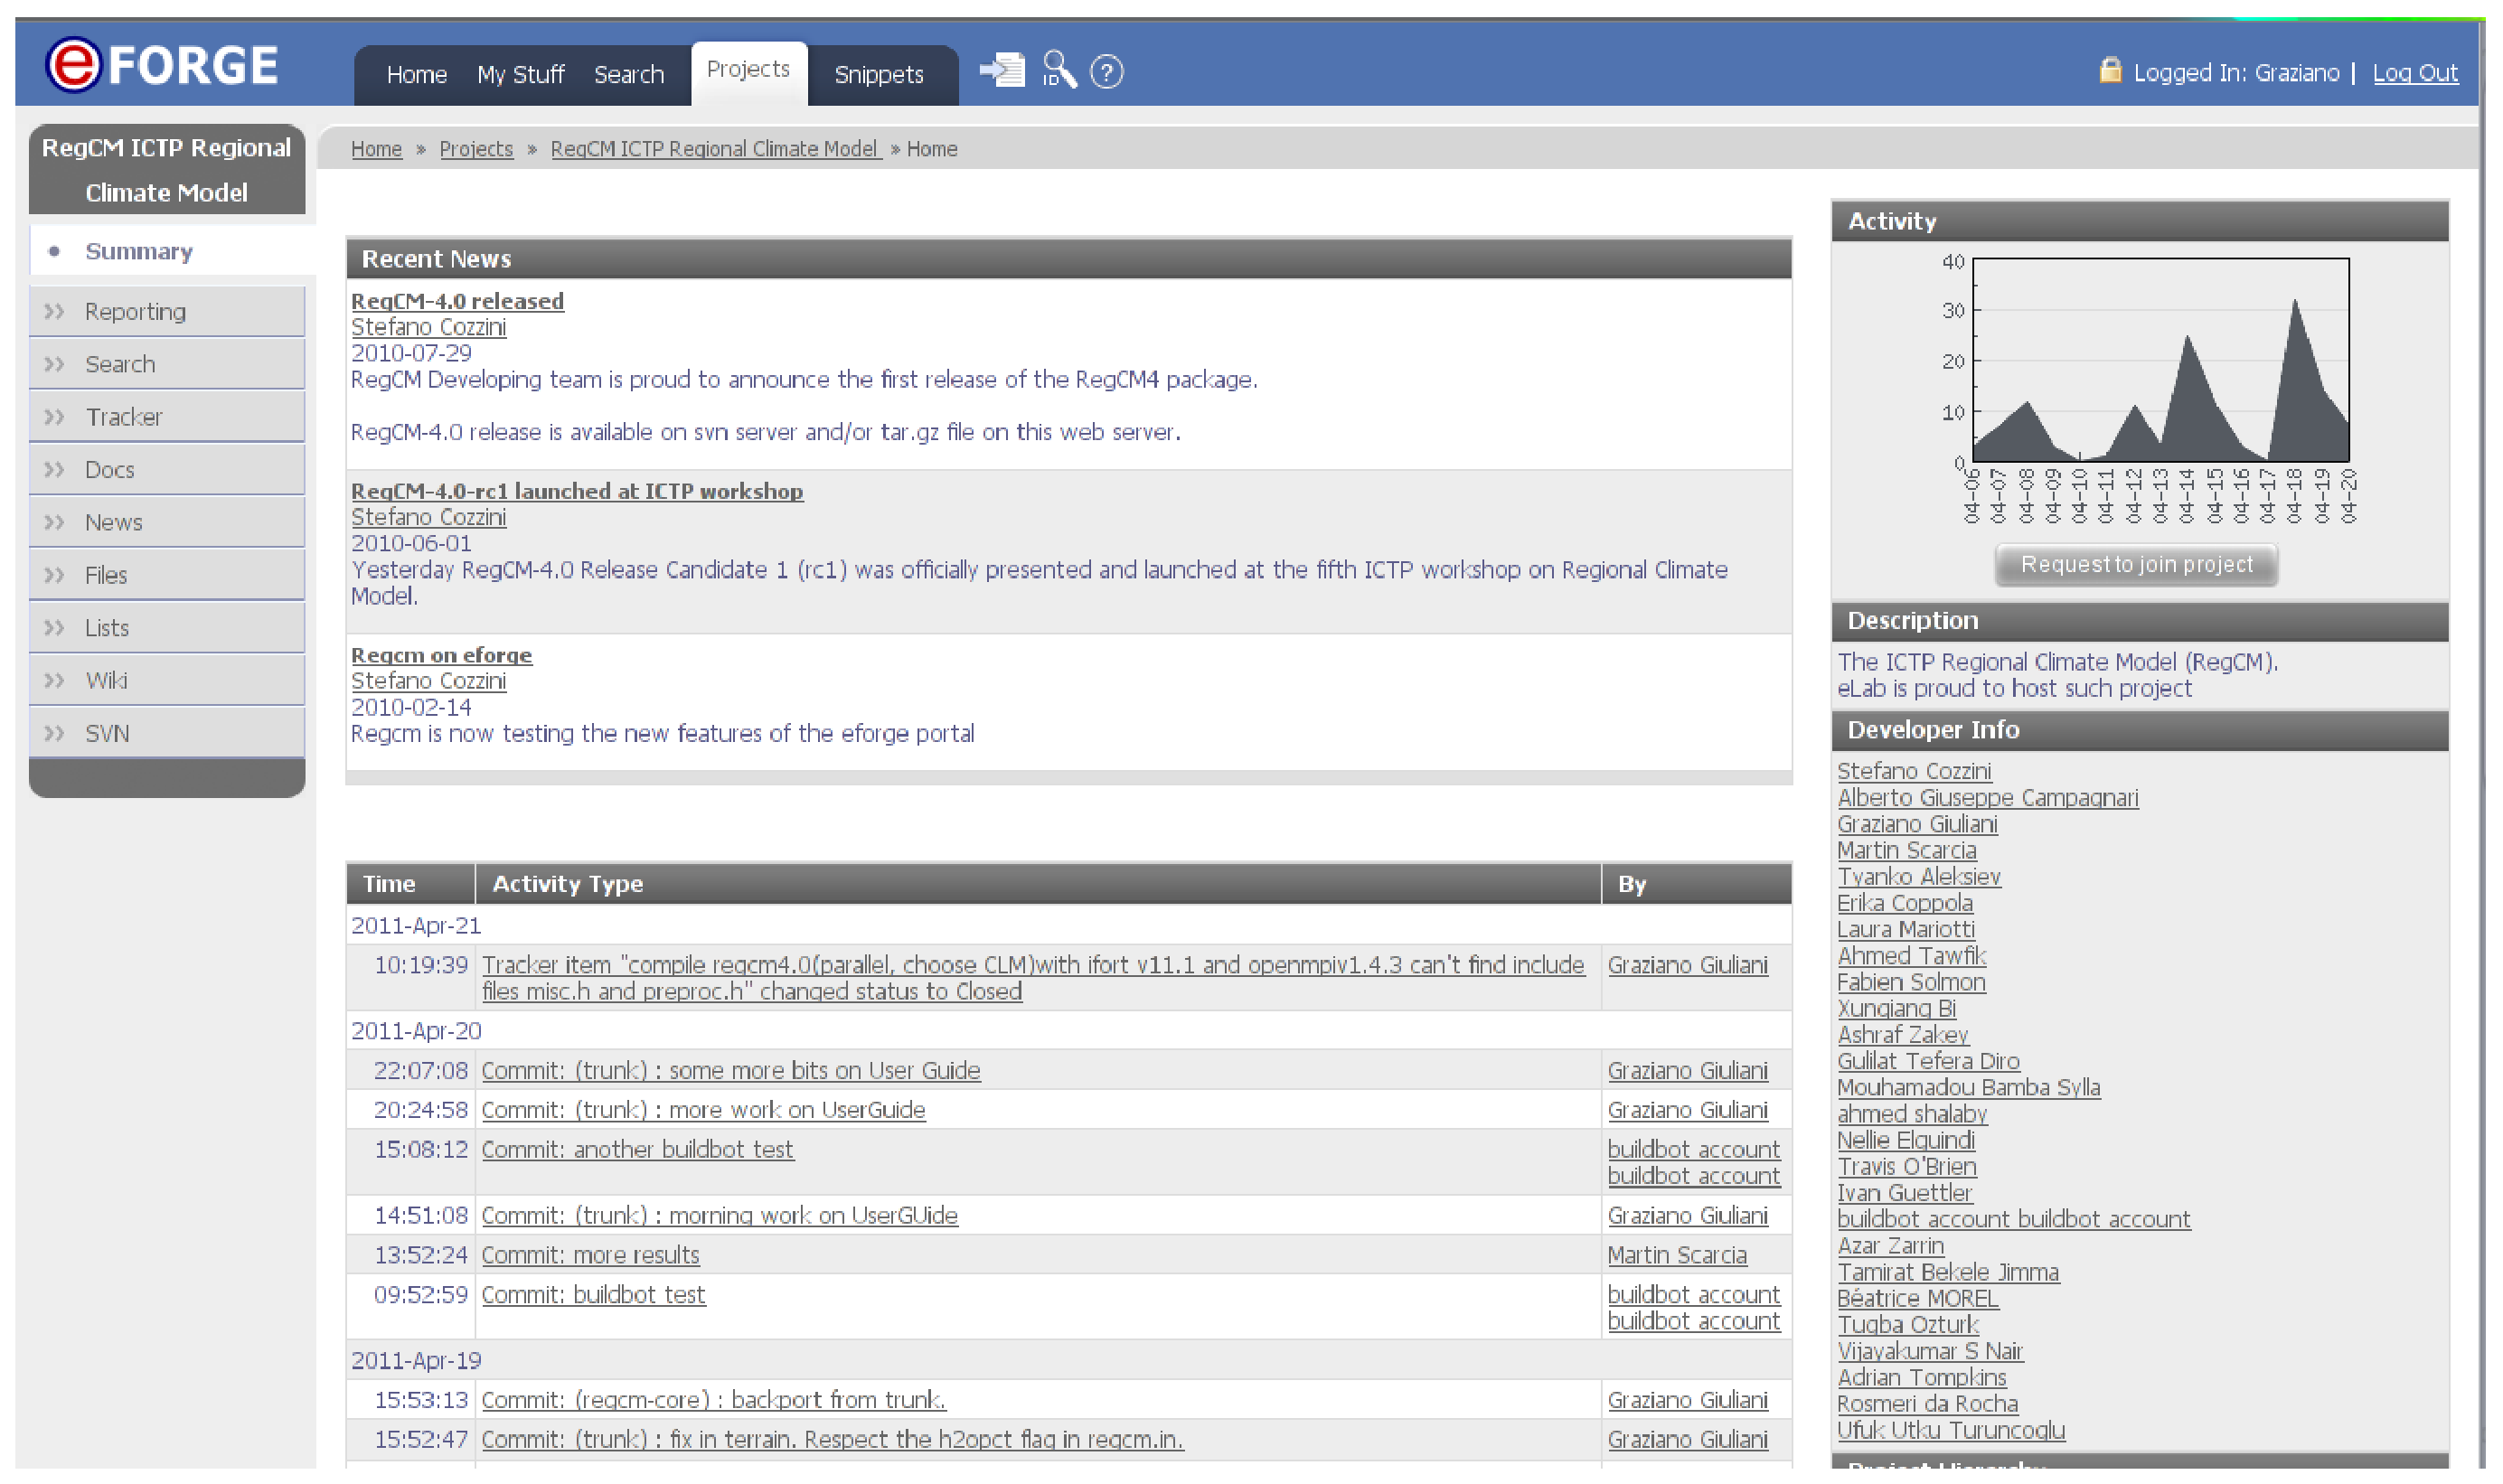
\includegraphics[width=12cm]{e-forge}
\end{figure}

On this site you have access with a simple registration to a friendly
bug tracking system under the {\em tracker} link, allowing the users to
post problems and bugs they discover.

It allows posting also of files to give you the opportunity to provide as
much information as possible about the environment the model is running at
your institution, helping us better understand and solve efficiently your
problems.

Help us grow the model to fit your requirements, giving the broader user
community the benefit of a valuable tool to do better research.

\newpage

\cleardoublepage

\chapter{Appendices}
\label{Appendice}
%
% This file is part of ICTP RegCM model.
% Copyright (C) 2011 ICTP Trieste
% See the file COPYING for copying conditions.
%

We will review here a sample installation session of software needed to
install the RegCM model.

The starting point is here a Linux system on a multicore processor box, and
the final goal is to have an optimized system to run the model.
I will use \verb=bash= as my shell and assume that GNU development tools like
\verb=make=, \verb=sed=, \verb=awk= are installed as part of the default
Operating System environment as is the case in most Linux distro.
I will require also for commodity a command line web downloader such as
\verb=curl= installed on the system, along its development libraries to be
used to enable OpenDAP remote data access protocol capabilities of netCDF
library. Standard file management tools such as \verb=tar= and \verb=gzip=
and \verb=wget= are also required.
The symbol \verb=$>= will stand for a shell prompt.
I will assume that the process is performed as a normal system user, which
will own all the toolchain. I will be now just the \verb=regcm= user.

\section{Identify Processor}

First step is to identify the processor to know its capabilities:

\begin{Verbatim}
$> cat /proc/cpuinfo
\end{Verbatim}

This command will ask to the operating system to print processor informations.
A sample answer on my laptop is:

\begin{Verbatim}
processor       : 0
vendor_id       : GenuineIntel
cpu family      : 6
model           : 30
model name      : Intel(R) Core(TM) i7 CPU       Q 740  @ 1.73GHz
stepping        : 5
cpu MHz         : 933.000
cache size      : 6144 KB
physical id     : 0
siblings        : 8
core id         : 0
cpu cores       : 4
apicid          : 0
initial apicid  : 0
fpu             : yes
fpu_exception   : yes
cpuid level     : 11
wp              : yes
flags           : fpu vme de pse tsc msr pae mce cx8 apic sep mtrr pge
mca cmov pat pse36 clflush dts acpi mmx fxsr sse sse2 ss ht tm pbe syscall
nx rdtscp lm constant_tsc arch_perfmon pebs bts rep_good nopl xtopology
nonstop_tsc aperfmperf pni dtes64 monitor ds_cpl vmx smx est tm2 ssse3
cx16 xtpr pdcm sse4_1 sse4_2 popcnt lahf_lm ida dts tpr_shadow vnmi
flexpriority ept vpid
bogomips        : 3467.81                                                       
clflush size    : 64                                                            
cache_alignment : 64                                                            
address sizes   : 36 bits physical, 48 bits virtual                             
power management:
\end{Verbatim}

repeated eight time with Processor Ids from 0 to 7: I have a Quad Core Intel
with Hyperthreading on (this multiply by 2 the reported processor list).
The processor reports here also to support Intel Streaming SIMD Extensions V4.2,
which can be later used to speed up code execution vectorizing floating point
operation on any single CPU core.

\section{Chose compiler}

Depending on the processor, we can chose which compiler to use. On a Linux box,
we have multiple choices:

\begin{itemize}
\item GNU Gfortran
\item G95
\item Intel ifort compiler
\item Portland pgf90 compiler
\item Absoft ProFortran
\item NAG Fortran Compiler
\end{itemize}

and for sure other which I may not be aware of. All of these compilers have pros
and cons, so I am just for now selecting one in the pool only to continue the
exposition. I am not selecting the trivial solution of Gfortran as most
Linux distributions have it already packaged, and all the other required
software as well (most complete distribution I am aware of for this is Fedora:
all needed software is packaged and it is a matter of yum install).

So let us assume I have licensed the Intel Composer XE Professional Suite
13.0.0 on my laptop. My system administrator installed it on the default
location under \verb=/opt/intel=, and I have my shell environment update
loading vendor provided script:

\begin{Verbatim}
$> source /opt/intel/bin/compilervars.sh intel64
\end{Verbatim}

With some modification (the path, the script, the arguments to the script),
same step is to be performed for all non-GNU compilers in the above list, and
is documented in the installation manual of the compiler itself.

In case of Intel, to check the correct behaviour of the compiler, try to
type the following command:

\begin{Verbatim}
$> ifort --version
ifort (IFORT) 13.0.0 20120731
Copyright (C) 1985-2012 Intel Corporation.  All rights reserved.
\end{Verbatim}

I am skipping here any problem that may arise from license installation for any
of the compilers, so I am assuming that if the compiler is callable, it works.
As this step is usually performed by a system administrator on the machine,
I am assuming a skilled professional will take care of that.

\section{Environment setup}

To efficiently use the compilers, I will setup now some environment variables.
On my system (see the above processor informations) I will use:

\begin{Verbatim}
$> # Where all the software will be installed ?
$> # I am chosing here a place under my home directory.
$> export INTELROOT=/home/regcm/intelsoft
$> # the C compiler. I am assuming here to have the whole Intel
$> # Composer XE suite, so I will use the intel C compiler.
$> export CC=icc
$> # the C++ compiler, the intel one.
$> export CXX=icpc
$> # the Fortran 9X compiler.
$> export FC=ifort
$> # the Foirtran 77 compiler. For intel, is just the fortran one.
$> export F77=ifort
$> # C Compiler flags
$> export CFLAGS="-O3 -xHost -axSSE4.2 -fPIC"
$> # F9X Compiler flags
$> export FCFLAGS="-O3 -xHost -axSSE4.2 -fPIC"
$> # F77 Compiler flags
$> export FFLAGS="-O3 -xHost -axSSE4.2 -fPIC"
$> # CXX Compiler flags
$> export CXXFLAGS="-O3 -xHost -axSSE4.2 -fPIC"
$> # Linker flags
$> export LDFLAGS="-Wl,-rpath=$INTELROOT/lib \
> -Wl,-rpath=/opt/intel/lib/intel64 -i-dynamic"
$> # Preset PATH to use the installed software during build
$> export PATH=$INTELROOT/bin:$PATH
$> export LD_LIBRARY_PATH=$LD_LIBRARY_PATH:$INTELROOT/lib
$> export MANPATH=$INTELROOT/share/man:$MANPATH
\end{Verbatim}

This step will allow me not to specify those variables at every following step.
Depending on the above compiler selected, those flags my differ for you, but the
concept is that I am selecting a performance target build for the machine I am
on. I am now ready to compile software.

\section{Pre requisite library installation}

To build a complete optimized stack, a sample script have been added
in \verb=Tools/Script/prereq_install.sh=
This help script will build netCDF V4 and MPICH2 libraries to be used to
compile the RegCM model.
Following the above settings, the script must be edited in the first lines
setting the \verb=DEST= variable to \verb=$INTELROOT=.

Then we can just execute the script:

\begin{Verbatim}
$> ./prereq_install.sh
This script installs the netCDF/mpi librares in the:
    /home/regcm/intelsoft
directory.
If something goes wrong, logs are saved in:
    /home/regcm/intelsoft/logs
Downloading ZLIB library...
Downloading HDF5 library...
Downloading netCDF Library...
Downloading MPICH2 Library...
Compiling MPI2 library.
Compiled MPI2 library.
Compiling zlib Library.
Compiled Zlib library.
Compiling HDF5 library.
Compiled HDF5 library.
Compiling netCDF Library.
Compiled netCDF C library.
Done!
To link RegCM with this librares use:

PATH=/home/regcm/intelsoft/bin:$PATH ./configure \
  CC=icc FC=ifort \
  CPPFLAGS=-I/home/regcm/intelsoft/include \
  LDFLAGS=-L/home/regcm/intelsoft/lib \
  LIBS="-lnetcdff -lnetcdf -lhdf5_hl -lhdf5 -lz"

\end{Verbatim}

The admins who must compile the pre requisite libraries are invited to look
at the script, identifying the various steps.
The normal user should be content of the last printout message which details
how to use the just built libraries to compile RegCM model sources against.
At run time an environment variable must be added to set correct paths:

\begin{Verbatim}
$> export PATH=/home/regcm/intelsoft/bin:$PATH
\end{Verbatim}


\newpage

\bibliography{references}
\bibliographystyle{agu}

\cleardoublepage

\evensidemargin=1.0cm
\oddsidemargin=1.5cm
\VerbatimInput[fontfamily=courier,fontsize=\footnotesize]{COPYING}

\end{document}
